\documentclass[twoside,11pt]{article}

% ? Specify used packages
\usepackage{graphicx}        %  Use this one for final production.
% \usepackage[draft]{graphicx} %  Use this one for drafting.
% ? End of specify used packages

\pagestyle{myheadings}

% -----------------------------------------------------------------------------
% ? Document identification
% Fixed part
\newcommand{\stardoccategory}  {Starlink User Note}
\newcommand{\stardocinitials}  {SUN}
\newcommand{\stardocsource}    {sun\stardocnumber}
\newcommand{\stardoccopyright}
{Copyright \copyright\ 2012 University of British Columbia and the Science \& Technology Facilities Council}

% Variable part - replace [xxx] as appropriate.
\newcommand{\stardocnumber}    {264.0}
\newcommand{\stardocauthors}   {Andrew G. Gibb \& Tim Jenness}
\newcommand{\stardocdate}      {27 July 2012}
\newcommand{\stardoctitle}     {ORAC-DR --- SCUBA-2 Pipeline Data Reduction}
\newcommand{\stardocversion}   {Version 1.1.0}
\newcommand{\stardocmanual}    {User's Guide}
\newcommand{\stardocabstract}  {

  The \oracdr\ data reduction pipeline is designed to reduce data from
  many different instruments. This document describes how to use
  \oracdr\ to process data taken with the SCUBA-2 instrument on the
  James Clerk Maxwell Telescope.

}
% ? End of document identification
% -----------------------------------------------------------------------------

% +
%  Name:
%     sun264.tex
%
%  Purpose:
%     Documentation for SCUBA-2 data reduction with ORAC-DR
%
%  Authors:
%     AGG: Andy Gibb (UBC)
%
%  History:
%     2010-10-26 (AGG):
%        Initial version
%     2012-07-25 (AGG):
%        Updates for Kapuahi
%     {Add further history here}
%
% -

\newcommand{\stardocname}{\stardocinitials /\stardocnumber}
\markboth{\stardocname}{\stardocname}
\setlength{\textwidth}{160mm}
\setlength{\textheight}{230mm}
\setlength{\topmargin}{-2mm}
\setlength{\oddsidemargin}{0mm}
\setlength{\evensidemargin}{0mm}
\setlength{\parindent}{0mm}
\setlength{\parskip}{\medskipamount}
\setlength{\unitlength}{1mm}

% -----------------------------------------------------------------------------
%  Hypertext definitions.
%  ======================
%  These are used by the LaTeX2HTML translator in conjunction with star2html.

%  Comment.sty: version 2.0, 19 June 1992
%  Selectively in/exclude pieces of text.
%
%  Author
%    Victor Eijkhout                                      <eijkhout@cs.utk.edu>
%    Department of Computer Science
%    University Tennessee at Knoxville
%    104 Ayres Hall
%    Knoxville, TN 37996
%    USA

%  Do not remove the %begin{latexonly} and %end{latexonly} lines (used by
%  LaTeX2HTML to signify text it shouldn't process).
%begin{latexonly}
\makeatletter
\def\makeinnocent#1{\catcode`#1=12 }
\def\csarg#1#2{\expandafter#1\csname#2\endcsname}

\def\ThrowAwayComment#1{\begingroup
    \def\CurrentComment{#1}%
    \let\do\makeinnocent \dospecials
    \makeinnocent\^^L% and whatever other special cases
    \endlinechar`\^^M \catcode`\^^M=12 \xComment}
{\catcode`\^^M=12 \endlinechar=-1 %
 \gdef\xComment#1^^M{\def\test{#1}
      \csarg\ifx{PlainEnd\CurrentComment Test}\test
          \let\html@next\endgroup
      \else \csarg\ifx{LaLaEnd\CurrentComment Test}\test
            \edef\html@next{\endgroup\noexpand\end{\CurrentComment}}
      \else \let\html@next\xComment
      \fi \fi \html@next}
}
\makeatother

\def\includecomment
 #1{\expandafter\def\csname#1\endcsname{}%
    \expandafter\def\csname end#1\endcsname{}}
\def\excludecomment
 #1{\expandafter\def\csname#1\endcsname{\ThrowAwayComment{#1}}%
    {\escapechar=-1\relax
     \csarg\xdef{PlainEnd#1Test}{\string\\end#1}%
     \csarg\xdef{LaLaEnd#1Test}{\string\\end\string\{#1\string\}}%
    }}

%  Define environments that ignore their contents.
\excludecomment{comment}
\excludecomment{rawhtml}
\excludecomment{htmlonly}

%  Hypertext commands etc. This is a condensed version of the html.sty
%  file supplied with LaTeX2HTML by: Nikos Drakos <nikos@cbl.leeds.ac.uk> &
%  Jelle van Zeijl <jvzeijl@isou17.estec.esa.nl>. The LaTeX2HTML documentation
%  should be consulted about all commands (and the environments defined above)
%  except \xref and \xlabel which are Starlink specific.

\newcommand{\htmladdnormallinkfoot}[2]{#1\footnote{#2}}
\newcommand{\htmladdnormallink}[2]{#1}
\newcommand{\htmladdimg}[1]{}
\newcommand{\hyperref}[4]{#2\ref{#4}#3}
\newcommand{\htmlref}[2]{#1}
\newcommand{\htmlimage}[1]{}
\newcommand{\htmladdtonavigation}[1]{}

\newenvironment{latexonly}{}{}
\newcommand{\latex}[1]{#1}
\newcommand{\html}[1]{}
\newcommand{\latexhtml}[2]{#1}
\newcommand{\HTMLcode}[2][]{}

%  Starlink cross-references and labels.
\newcommand{\xref}[3]{#1}
\newcommand{\xlabel}[1]{}

%  LaTeX2HTML symbol.
\newcommand{\latextohtml}{\LaTeX2\texttt{HTML}}

%  Define command to re-centre underscore for Latex and leave as normal
%  for HTML (severe problems with \_ in tabbing environments and \_\_
%  generally otherwise).
\renewcommand{\_}{\texttt{\symbol{95}}}

% -----------------------------------------------------------------------------
%  Debugging.
%  =========
%  Remove % on the following to debug links in the HTML version using Latex.

% \newcommand{\hotlink}[2]{\fbox{\begin{tabular}[t]{@{}c@{}}#1\\\hline{\footnotesize #2}\end{tabular}}}
% \renewcommand{\htmladdnormallinkfoot}[2]{\hotlink{#1}{#2}}
% \renewcommand{\htmladdnormallink}[2]{\hotlink{#1}{#2}}
% \renewcommand{\hyperref}[4]{\hotlink{#1}{\S\ref{#4}}}
% \renewcommand{\htmlref}[2]{\hotlink{#1}{\S\ref{#2}}}
% \renewcommand{\xref}[3]{\hotlink{#1}{#2 -- #3}}
%end{latexonly}
% -----------------------------------------------------------------------------
% ? Document specific \newcommand or \newenvironment commands.

% A new environment for quoting verbatim
% Environment for indenting and using a small font.
\newenvironment{myquote}{\begin{quote}\begin{small}}{\end{small}\end{quote}}

\newcommand{\starlink}{\htmladdnormallink{Starlink}{http://starlink.jach.hawaii.edu}}

% Shorthand and HTML references for other Starlink tasks
\newcommand{\CCDPACK}{\textsc{ccdpack}}
\newcommand{\CCDPACKref}{\xref{\CCDPACK}{sun139}{}}
\newcommand{\CUPID}{\textsc{cupid}}
\newcommand{\CUPIDref}{\xref{\CUPID}{sun255}{}}
\newcommand{\FLUXES}{\textsc{fluxes}}
\newcommand{\FLUXESref}{\xref{\FLUXES}{sun213}{}}
\newcommand{\GAIA}{\textsc{gaia}}
\newcommand{\GAIAref}{\xref{\GAIA}{sun214}{}}
\newcommand{\HDSTRACE}{\textsc{hdstrace}}
\newcommand{\HDSTRACEref}{\xref{\HDSTRACE}{sun102}{}}
\newcommand{\KAPPA}{\textsc{kappa}}
\newcommand{\CURSA}{\xref{\textsc{cursa}}{sun190}{}}
\newcommand{\KAPPAref}{\xref{(SUN/95)}{sun95}{}}
\newcommand{\SMURF}{\textsc{smurf}}
\newcommand{\SMURFcook}{\xref{SC/19}{sc19}{}}
\newcommand{\SMURFsun}{\xref{SUN/258}{sun258}{}}
\newcommand{\ADAMsgref}{\xref{SG/4}{sg4}{}}
\newcommand{\ADAMsunref}{\xref{SUN/101}{sun101}{}}
\newcommand{\astref}{\xref{SUN/211}{sun211}{}}
\newcommand{\ndfref}{\xref{SUN/33}{sun33}{}}

\newcommand{\oracdr}{\textsc{orac-dr}}
\newcommand{\oracsun}{\xref{SUN/230}{sun230}{}}
\newcommand{\scubasun}{\xref{SUN/231}{sun231}{}}
\newcommand{\picard}{\textsc{picard}}
\newcommand{\picardsun}{\xref{SUN/265}{sun265}{}}

% Application tasks
\newcommand{\task}[1]{\textsf{#1}}

% SMURF tasks
\newcommand{\badbolos}{\xref{\task{badbolos}}{sun258}{BADBOLOS}}
\newcommand{\calcdark}{\xref{\task{calcdark}}{sun258}{CALCDARK}}
\newcommand{\calcflat}{\xref{\task{calcflat}}{sun258}{CALCFLAT}}
\newcommand{\calcnoise}{\xref{\task{calcnoise}}{sun258}{CALCNOISE}}
\newcommand{\calcresp}{\xref{\task{calcresp}}{sun258}{CALCRESP}}
\newcommand{\copyflat}{\xref{\task{copyflat}}{sun258}{COPYFLAT}}
\newcommand{\dreamsolve}{\xref{\task{dreamsolve}}{sun258}{DREAMSOLVE}}
\newcommand{\dreamweights}{\xref{\task{dreamweights}}{sun258}{DREAMWEIGHTS}}
\newcommand{\gsdtoacsis}{\xref{\task{gsd2acsis}}{sun258}{GSD2ACSIS}}
\newcommand{\gsdshow}{\xref{\task{gsdshow}}{sun258}{GSDSHOW}}
\newcommand{\smurfhelp}{\xref{\task{smurfhelp}}{sun258}{SMURFHELP}}
\newcommand{\impaztec}{\xref{\task{impaztec}}{sun258}{IMPAZTEC}}
\newcommand{\makecube}{\xref{\task{makecube}}{sun258}{MAKECUBE}}
\newcommand{\qlmakemap}{\xref{\task{qlmakemap}}{sun258}{QLMAKEMAP}}
\newcommand{\rawunpress}{\xref{\task{rawunpress}}{sun258}{RAWUNPRESS}}
\newcommand{\rawfixmeta}{\xref{\task{rawfixmeta}}{sun258}{RAWFIXMETA}}
\newcommand{\sctwosim}{\xref{\task{sc2sim}}{sun258}{SC2SIM}}
\newcommand{\sctwothreadtest}{\xref{\task{sc2threadtest}}{sun258}{SC2THREADTEST}}
\newcommand{\scanfit}{\xref{\task{scanfit}}{sun258}{SCANFIT}}
\newcommand{\skynoise}{\xref{\task{skynoise}}{sun258}{SKYNOISE}}
\newcommand{\smurfcopy}{\xref{\task{smurfcopy}}{sun258}{SMURFCOPY}}
\newcommand{\stackframes}{\xref{\task{stackframes}}{sun258}{STACKFRAMES}}
\newcommand{\starecalc}{\xref{\task{starecalc}}{sun258}{STARECALC}}
\newcommand{\timesort}{\xref{\task{timesort}}{sun258}{TIMESORT}}
\newcommand{\unmakecube}{\xref{\task{unmakecube}}{sun258}{UNMAKECUBE}}

\newcommand{\extinction}{\xref{\task{extinction}}{sun258}{EXTINCTION}}
\newcommand{\flatfield}{\xref{\task{flatfield}}{sun258}{FLATFIELD}}
\newcommand{\jcmtstate}{\xref{\task{jcmtstate2cat}}{sun258}{JCMTSTATE2CAT}}
\newcommand{\dumpocscfg}{\xref{\task{dumpocscfg}}{sun258}{DUMPOCSCFG}}
\newcommand{\makemap}{\xref{\task{makemap}}{sun258}{MAKEMAP}}
\newcommand{\gettsys}{\xref{\task{gettsys}}{sun258}{GETTSYS}}

\newcommand{\remsky}{\xref{\task{remsky}}{sun258}{REMSKY}}
\newcommand{\clean}{\xref{\task{sc2clean}}{sun258}{SC2CLEAN}}
\newcommand{\concat}{\xref{\task{sc2concat}}{sun258}{SC2CONCAT}}
\newcommand{\fft}{\xref{\task{sc2fft}}{sun258}{SC2FFT}}
\newcommand{\fts}{\xref{\task{sc2fts}}{sun258}{SC2FTS}}

\newcommand{\rebin}{\texttt{rebin}}
\newcommand{\iterate}{\texttt{iterate}}

% Other tasks
\newcommand{\makemos}{\xref{\task{makemos}}{sun139}{MAKEMOS}}
\newcommand{\csub}{\xref{\task{csub}}{sun95}{CSUB}}
\newcommand{\clinplot}{\xref{\task{clinplot}}{sun95}{CLINPLOT}}
\newcommand{\mlinplot}{\xref{\task{mlinplot}}{sun95}{MLINPLOT}}
\newcommand{\collapse}{\xref{\task{collapse}}{sun95}{COLLAPSE}}
\newcommand{\fitsedit}{\xref{\task{fitsedit}}{sun95}{FITSEDIT}}
\newcommand{\kapdiv}{\xref{\task{div}}{sun95}{DIV}}
\newcommand{\ndfcopy}{\xref{\task{ndfcopy}}{sun95}{NDFCOPY}}
\newcommand{\provshow}{\xref{\task{provshow}}{sun95}{PROVSHOW}}
\newcommand{\thresh}{\xref{\task{thresh}}{sun95}{THRESH}}
\newcommand{\wcsmosaic}{\xref{\task{wcsmosaic}}{sun95}{WCSMOSAIC}}
\newcommand{\wcsalign}{\xref{\task{wcsalign}}{sun95}{WCSALIGN}}
\newcommand{\wcsattrib}{\xref{\task{wcsattrib}}{sun95}{WCSATTRIB}}
\newcommand{\fitslist}{\xref{\task{fitslist}}{sun95}{FITSLIST}}
\newcommand{\display}{\xref{\task{display}}{sun95}{DISPLAY}}
\newcommand{\topcat}{\xref{\textsc{Topcat}}{sun253}{}}


% macros for typesetting parameters
\newcommand{\aparam}[1]{\texttt{#1}}     % ADAM parameter
\newcommand{\cparam}[1]{\texttt{#1}}     % CONFIG parameter
\newcommand{\ndfcomp}[1]{\texttt{#1}}    % NDF component

%% Definitions imported from SUN/95

% A kind of list item, like description, but with an easily adjustable
% item separation.  Note that the paragraph and fount-size change are
% needed to make the revised \baselinestretch work.
\newlength{\menuwidth}
\newlength{\menuindent}
\newcommand{\menuitem}[2]
  {{\bf #1} \settowidth{\menuwidth}{{\bf #1} }
  \setlength{\menuindent}{-0.5em}
  \addtolength{\menuwidth}{-2\menuwidth}
  \addtolength{\menuwidth}{\textwidth}
  \addtolength{\menuwidth}{\menuindent}
  \hspace{\menuindent}\parbox[t]{\menuwidth}{
  \renewcommand{\baselinestretch}{0.75}\small
  #2 \par \vspace{1.0ex}
  \renewcommand{\baselinestretch}{1.0}\normalsize} \\ }
\begin{htmlonly}
\newcommand{\menuitem}[2]
  {\item [\htmlref{#1}{#1}] #2}
\end{htmlonly}

\newcommand{\classitem}[1]{\item [\htmlref{#1}{#1}]}

% an environment for references (for the SST sstdiytopic command).
\newenvironment{refs}{\vspace{-4ex} % normally 3ex
                      \begin{list}{}{\setlength{\topsep}{0mm}
                                     \setlength{\partopsep}{0mm}
                                     \setlength{\itemsep}{0mm}
                                     \setlength{\parsep}{0mm}
                                     \setlength{\leftmargin}{1.5em}
                                     \setlength{\itemindent}{-\leftmargin}
                                     \setlength{\labelsep}{0mm}
                                     \setlength{\labelwidth}{0mm}}
                    }{\end{list}}

%+
%  Name:
%     SST.TEX

%  Purpose:
%     Define LaTeX commands for laying out Starlink routine descriptions.

%  Language:
%     LaTeX

%  Type of Module:
%     LaTeX data file.

%  Description:
%     This file defines LaTeX commands which allow routine documentation
%     produced by the SST application PROLAT to be processed by LaTeX and
%     by LaTeX2html. The contents of this file should be included in the
%     source prior to any statements that make of the sst commnds.

%  Notes:
%     The style file html.sty provided with LaTeX2html needs to be used.
%     This must be before this file.

%  Authors:
%     RFWS: R.F. Warren-Smith (STARLINK)
%     PDRAPER: P.W. Draper (Starlink - Durham University)

%  History:
%     10-SEP-1990 (RFWS):
%        Original version.
%     10-SEP-1990 (RFWS):
%        Added the implementation status section.
%     12-SEP-1990 (RFWS):
%        Added support for the usage section and adjusted various spacings.
%     8-DEC-1994 (PDRAPER):
%        Added support for simplified formatting using LaTeX2html.
%     21-JUL-2009 (TIMJ):
%        Added \sstdiylist{}{} as used when a Parameters section is located that
%        is not "ADAM Parameters".
%     {enter_further_changes_here}

%  Bugs:
%     {note_any_bugs_here}

%-

%  Define length variables.
\newlength{\sstbannerlength}
\newlength{\sstcaptionlength}
\newlength{\sstexampleslength}
\newlength{\sstexampleswidth}

%  Define a \tt font of the required size.
\latex{\newfont{\ssttt}{cmtt10 scaled 1095}}
\html{\newcommand{\ssttt}{\tt}}

%  Define a command to produce a routine header, including its name,
%  a purpose description and the rest of the routine's documentation.
\newcommand{\sstroutine}[3]{
   \goodbreak
   \rule{\textwidth}{0.5mm}
   \vspace{-7ex}
   \newline
   \settowidth{\sstbannerlength}{{\Large {\bf #1}}}
   \setlength{\sstcaptionlength}{\textwidth}
   \setlength{\sstexampleslength}{\textwidth}
   \addtolength{\sstbannerlength}{0.5em}
% Modifications to only print title once: see SUN232 for info
   \addtolength{\sstcaptionlength}{-1.0\sstbannerlength}
   \addtolength{\sstcaptionlength}{-2.5pt}
   \settowidth{\sstexampleswidth}{{\bf Examples:}}
   \addtolength{\sstexampleslength}{-\sstexampleswidth}
   \parbox[t]{\sstbannerlength}{\flushleft{\Large {\bf #1}}}
   \parbox[t]{\sstcaptionlength}{\center{\Large #2}}
%   \parbox[t]{\sstbannerlength}{\flushright{\Large {\bf #1}}}
   \begin{description}
      #3
   \end{description}
}

%  Format the description section.
\newcommand{\sstdescription}[1]{\item[Description:] #1}

%  Format the usage section.
\newcommand{\sstusage}[1]{\item[Usage:] \mbox{}
\\[1.3ex]{\raggedright \ssttt #1}}

%  Format the invocation section.
\newcommand{\sstinvocation}[1]{\item[Invocation:]\hspace{0.4em}{\tt #1}}

%  Format the arguments section.
\newcommand{\sstarguments}[1]{
   \item[Arguments:] \mbox{} \\
   \vspace{-3.5ex}
   \begin{description}
      #1
   \end{description}
}

%  Format the returned value section (for a function).
\newcommand{\sstreturnedvalue}[1]{
   \item[Returned Value:] \mbox{} \\
   \vspace{-3.5ex}
   \begin{description}
      #1
   \end{description}
}

%  Format the parameters section (for an application).
\newcommand{\sstparameters}[1]{
   \item[Parameters:] \mbox{} \\
   \vspace{-3.5ex}
   \begin{description}
      #1
   \end{description}
}

%  Format the examples section.
\newcommand{\sstexamples}[1]{
   \item[Examples:] \mbox{} \\
   \vspace{-3.5ex}
   \begin{description}
      #1
   \end{description}
}

%  Define the format of a subsection in a normal section.
\newcommand{\sstsubsection}[1]{ \item[{#1}] \mbox{} \\}

%  Define the format of a subsection in the examples section.
\newcommand{\sstexamplesubsection}[2]{\sloppy
\item[\parbox{\sstexampleslength}{\ssttt #1}] \mbox{} \vspace{1.0ex}
\\ #2 }

%  Format the notes section.
\newcommand{\sstnotes}[1]{\item[Notes:] \mbox{} \\[1.3ex] #1}

%  Provide a general-purpose format for additional (DIY) sections.
\newcommand{\sstdiytopic}[2]{\item[{\hspace{-0.35em}#1\hspace{-0.35em}:}]
\mbox{} \\[1.3ex] #2}

%  Format the a generic section as a list
\newcommand{\sstdiylist}[2]{
   \item[#1:] \mbox{} \\
   \vspace{-3.5ex}
   \begin{description}
      #2
   \end{description}
}

%  Format the implementation status section.
\newcommand{\sstimplementationstatus}[1]{
   \item[{Implementation Status:}] \mbox{} \\[1.3ex] #1}

%  Format the bugs section.
\newcommand{\sstbugs}[1]{\item[Bugs:] #1}

%  Format a list of items while in paragraph mode.
\newcommand{\sstitemlist}[1]{
  \mbox{} \\
  \vspace{-3.5ex}
  \begin{itemize}
     #1
  \end{itemize}
}

%  Define the format of an item.
\newcommand{\sstitem}{\item}

%% Now define html equivalents of those already set. These are used by
%  latex2html and are defined in the html.sty files.
\begin{htmlonly}

%  sstroutine.
   \newcommand{\sstroutine}[3]{
      \subsection{#1\xlabel{#1}-\label{#1}#2}
      \begin{description}
         #3
      \end{description}
   }

%  sstdescription
   \newcommand{\sstdescription}[1]{\item[Description:]
      \begin{description}
         #1
      \end{description}
      \\
   }

%  sstusage
   \newcommand{\sstusage}[1]{\item[Usage:]
      \begin{description}
         {\ssttt #1}
      \end{description}
      \\
   }

%  sstinvocation
   \newcommand{\sstinvocation}[1]{\item[Invocation:]
      \begin{description}
         {\ssttt #1}
      \end{description}
      \\
   }

%  sstarguments
   \newcommand{\sstarguments}[1]{
      \item[Arguments:] \\
      \begin{description}
         #1
      \end{description}
      \\
   }

%  sstreturnedvalue
   \newcommand{\sstreturnedvalue}[1]{
      \item[Returned Value:] \\
      \begin{description}
         #1
      \end{description}
      \\
   }

%  sstparameters
   \newcommand{\sstparameters}[1]{
      \item[Parameters:] \\
      \begin{description}
         #1
      \end{description}
      \\
   }

%  sstexamples
   \newcommand{\sstexamples}[1]{
      \item[Examples:] \\
      \begin{description}
         #1
      \end{description}
      \\
   }

%  sstsubsection
   \newcommand{\sstsubsection}[1]{\item[{#1}]}

%  sstexamplesubsection
   \newcommand{\sstexamplesubsection}[2]{\item[{\ssttt #1}] #2}

%  sstnotes
   \newcommand{\sstnotes}[1]{\item[Notes:] #1 }

%  sstdiytopic
   \newcommand{\sstdiytopic}[2]{\item[{#1}] #2 }

%  sstimplementationstatus
   \newcommand{\sstimplementationstatus}[1]{
      \item[Implementation Status:] #1
   }

%  sstitemlist
   \newcommand{\sstitemlist}[1]{
      \begin{itemize}
         #1
      \end{itemize}
      \\
   }
%  sstitem
   \newcommand{\sstitem}{\item}

\end{htmlonly}

%  End of "sst.tex" layout definitions.
%.



% ? End of document specific commands
% -----------------------------------------------------------------------------
%  Title Page.
%  ===========
\renewcommand{\thepage}{\roman{page}}
\begin{document}
\thispagestyle{empty}

%  Latex document header.
%  ======================
\begin{latexonly}
   \textsc{University of British Columbia} / \textsc{Joint Astronomy Centre} \hfill \textbf{\stardocname}\\
   {\large Science \& Technology Facilities Council}\\
   {\large Starlink Software Collection\\}
   {\large \stardoccategory\ \stardocnumber}
   \begin{flushright}
   \stardocauthors\\
   \stardocdate
   \end{flushright}
   \vspace{-4mm}
   \rule{\textwidth}{0.5mm}
   \vspace{5mm}
   \begin{center}
   {\Huge\textbf{\stardoctitle \\ [2.5ex]}}
   {\LARGE\textbf{\stardocversion \\ [4ex]}}
   {\Huge\textbf{\stardocmanual}}
   \end{center}
   \vspace{5mm}

% ? Add picture here if required for the LaTeX version.
%   e.g. \includegraphics[scale=0.3]{filename.ps}
\begin{center}
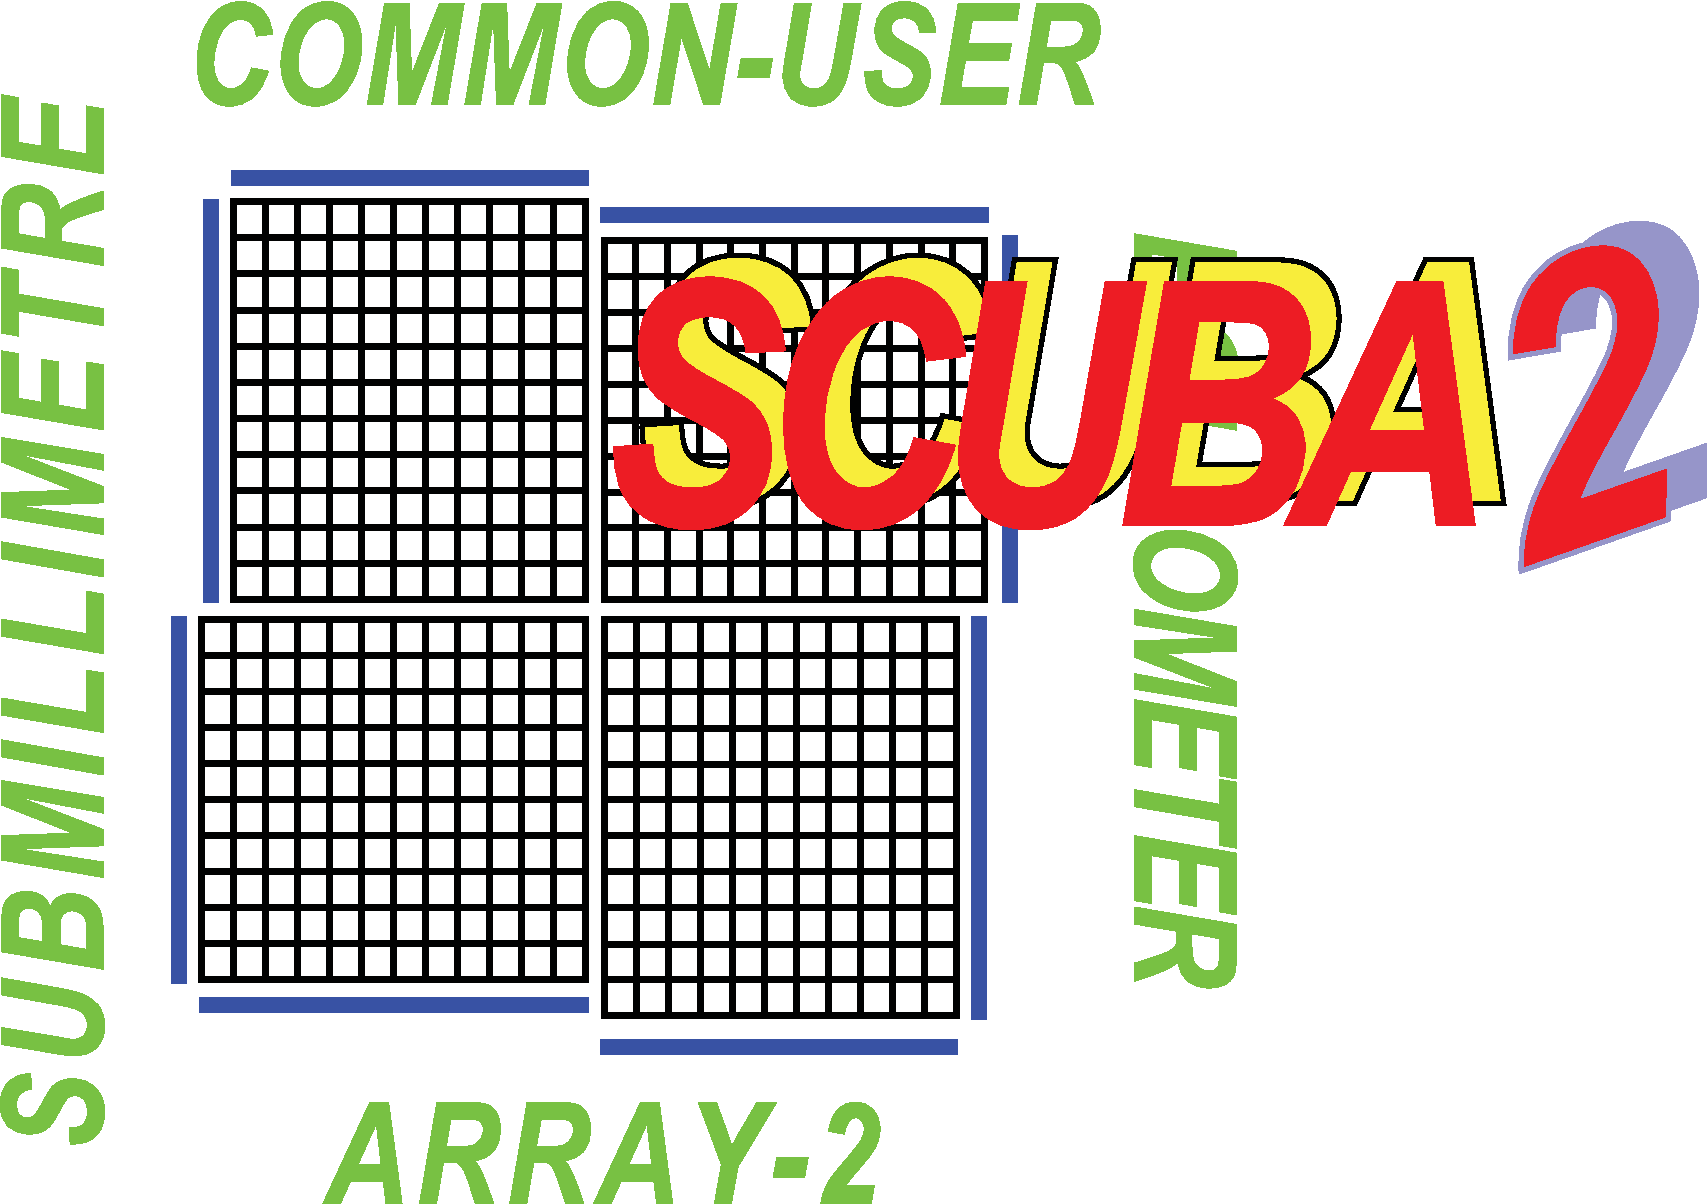
\includegraphics[scale=0.3]{sun264_logo}
\end{center}
% ? End of picture

% ? Heading for abstract if used.
   \vspace{10mm}
   \begin{center}
      {\Large\textbf{Abstract}}
   \end{center}
% ? End of heading for abstract.
\end{latexonly}

%  HTML documentation header.
%  ==========================
\begin{htmlonly}
   \xlabel{}
   \begin{rawhtml} <H1> \end{rawhtml}
      \stardoctitle\\
      \stardocversion\\
      \stardocmanual
   \begin{rawhtml} </H1> <HR> \end{rawhtml}

% ? Add picture here if required for the hypertext version.
%   e.g. \includegraphics[scale=0.7]{filename.ps}
\includegraphics[scale=0.7]{sun258_logo}
% ? End of picture

   \begin{rawhtml} <P> <I> \end{rawhtml}
   \stardoccategory\ \stardocnumber \\
   \stardocauthors \\
   \stardocdate
   \begin{rawhtml} </I> </P> <H3> \end{rawhtml}
      \htmladdnormallink{University of British Columbia}
                        {http://www.ubc.ca} \\
      \htmladdnormallink{Joint Astronomy Centre}
                        {http://www.jach.hawaii.edu}\\
      \htmladdnormallink{Science \& Technology Facilities Council}
                        {http://www.stfc.ac.uk} \\
   \begin{rawhtml} </H3> <H2> \end{rawhtml}
      \htmladdnormallink{Starlink Software Collection}{http://starlink.jach.hawaii.edu/}
   \begin{rawhtml} </H2> \end{rawhtml}
   \htmladdnormallink{\htmladdimg{source.gif} Retrieve hardcopy}
      {http://starlink.jach.hawaii.edu/cgi-bin/hcserver?\stardocsource}\\

%  HTML document table of contents.
%  ================================
%  Add table of contents header and a navigation button to return to this
%  point in the document (this should always go before the abstract \section).
  \label{stardoccontents}
  \begin{rawhtml}
    <HR>
    <H2>Contents</H2>
  \end{rawhtml}
  \htmladdtonavigation{\htmlref{\htmladdimg{contents_motif.gif}}
        {stardoccontents}}

% ? New section for abstract if used.
  \section{\xlabel{abstract}Abstract}
% ? End of new section for abstract
\end{htmlonly}

% -----------------------------------------------------------------------------
% ? Document Abstract. (if used)
%  ==================
\stardocabstract
% ? End of document abstract

% -----------------------------------------------------------------------------
% ? Latex Copyright Statement
%  =========================
\begin{latexonly}
\newpage
\vspace*{\fill}
\stardoccopyright
\end{latexonly}
% ? End of Latex copyright statement

% -----------------------------------------------------------------------------
% ? Latex document Table of Contents (if used).
%  ===========================================
  \newpage
  \begin{latexonly}
    \setlength{\parskip}{0mm}
    \tableofcontents
    \setlength{\parskip}{\medskipamount}
    \markboth{\stardocname}{\stardocname}
  \end{latexonly}
% ? End of Latex document table of contents
% -----------------------------------------------------------------------------

\cleardoublepage
\renewcommand{\thepage}{\arabic{page}}
\setcounter{page}{1}

% Main text

\section{\xlabel{introduction}Introduction\label{se:intro}}

The SCUBA-2 pipeline is a suite of recipes and primitives for the
\oracdr\ automated data processing software package. Additional
functionality for processing and analysis of reduced data is provided
through a number of \picard\ recipes. General documentation on
\oracdr\ and \picard\ can be found in \oracsun\ and
\picardsun\ respectively.

The fundamental operation of the pipeline is to begin with raw data
and produce calibrated science images with no additional user
input. All decisions are based on metadata stored in the data files
combined with basic quality assessment of reduced data products.

\subsection{Document conventions}

In an attempt to make this document clearer to read, different fonts
are used for specific structures.

Observing modes are denoted by all upper case body text (e.g.\
FLATFIELD).

Starlink package names are shown in small caps (e.g.\ \SMURF);
individual task names are shown in sans-serif
(e.g.\ \makemap). \oracdr\ recipes and primitives are also shown in
sans-serif and are always upper case (e.g.\ \task{REDUCE\_SCAN}).

Content listings are shown in fixed-width type (sometimes called
`typewriter'). Extensions and components within NDF (\ndfref) data
files are shown in upper case fixed-width type (e.g.\
\ndfcomp{HISTORY}).

Text relating to filenames (including suffices for data products), key
presses or entries typed at the command line are also denoted by
fixed-width type (e.g.\ \texttt{\% smurf}), as are parameters for
tasks which are displayed in upper case (e.g.\ \aparam{METHOD}).

References to Starlink documents, i.e., Starlink User Notes (SUN),
Starlink General documents (SG) and Starlink Cookbooks (SC), are given
in the text using the document type and the corresponding number
(e.g.\ SUN/95). Non-Starlink documents are cited in the text and
listed in the bibliography.

File name suffices represent the text between the final underscore
character and the three-letter \verb+.sdf+ extension. For example, a
file named \verb+s4a20101020_00002_0001_cal.sdf+ has the suffix
\verb+_cal+.

\section{\xlabel{pipelines}SCUBA-2 Pipeline Variants\label{se:pipelines}}

There are three variants of the SCUBA-2 pipeline, two of which are
designed to run in real time at the JCMT. Most users will only need to
run the third form, known as the science pipeline.

\begin{itemize}
\item The quick-look (QL) pipeline is primarily designed to perform
  quality-assurance analysis of the incoming data for real-time
  assessment of the instrument performance. It is also responsible for
  processing pointing and focus data.

\item The summit pipeline runs in parallel with the QL pipeline
  (though on a different machine) and is the primary image-processing
  pipeline. Processing is delayed until sufficient data exist to
  produce a higher quality image. In practice this happens after a
  certain time has elapsed since an image was last made.

\item The science pipeline has access to all the data observed for a
  given project and adopts a best-possible reduction approach. Images
  are made for each complete observation which are combined to create
  the final image.
\end{itemize}

\subsection{Requirements for running the SCUBA-2 pipeline}

The SCUBA-2 pipeline requires a recent Starlink installation. The
latest version may be obtained from
\htmladdnormallink{\texttt{http://starlink.jach.hawaii.edu/starlink}}{http://starlink.jach.hawaii.edu/starlink}. Since
development of the pipeline is an ongoing process, it is recommended
that the newest builds be used to access the full capabilities of the
pipeline. These builds can be obtained from\\
\htmladdnormallink{\texttt{http://starlink.jach.hawaii.edu/starlink/rsyncStarlink}}{http://starlink.jach.hawaii.edu/starlink/rsyncStarlink}
and may be kept up-to-date with rsync.

The Starlink Perl installation (Starperl) must be used to run the
pipeline due to the module requirements. The Starlink environment should be
initialized as usual before running \oracdr.

The software used to process raw data into images is called the
SubMillimetre User Reduction Facility (\SMURF). Detailed documentation
on \SMURF\ can be found in \SMURFsun, while \SMURFcook\ is a cookbook
that describes some of the background to SCUBA-2 data reduction.

The pipeline uses the following Starlink applications:
\begin{itemize}
\item \SMURF
\item \KAPPA
\item \FLUXES
\item \CCDPACK
\item \CUPID
\end{itemize}

\subsection{Important environment variables}

The pipeline uses a number of environment variables to determine where
data should be read from and written to. Some are set automatically
when the pipeline is initialized, but they can be overridden manually
and, with the \verb+-honour+ flag may be left unchanged between
successive runs of the pipeline. The variables that must be defined in
order for the pipelne to run are denoted as `Mandatory' in the list
below.

\begin{itemize}

\item \verb+STARLINK_DIR+: location of the user's Starlink
  installation. [Mandatory]

\item \verb+ORAC_DATA_IN+: the location where data are read from. If
  running with \verb+-loop flag+, this is the location of the flag
  files, rather than the data files. [Mandatory]

\item \verb+ORAC_DATA_OUT+: location where pipeline data products are
  written. Also used as a location for user-specified configuration
  files for \task{makemap}. [Mandatory]

\item \verb+ORAC_DATA_ROOT+: root location for data. At the JCMT,
  this is \verb+/jcmtdata/raw/scuba2+. If not defined, the current
  directory is assumed. [Optional]

\item \verb+MAKEMAP_CONFIG_DIR+: a user-specified location for
  \task{makemap} configuration files. [Optional]

\end{itemize}

\subsection{Getting help}

Basic help and a list of command-line options may be obtained after
initializing \oracdr\ by running :
\begin{myquote}
\begin{verbatim}
% oracdr -h
\end{verbatim}
\end{myquote}
or
\begin{myquote}
\begin{verbatim}
% oracdr -man
\end{verbatim}
\end{myquote}

More complete documentation on \oracdr\ can be found in \oracsun.

\section{\xlabel{runpipeline}Running the SCUBA-2 pipeline at the JCMT\label{se:runpipe}}

At the summit the pipeline is normally started by the telescope
support specialist (TSS) as normal user accounts do not have the
access privileges to write to the data output directories.

There are four pipelines running at the telescope, a QL and summit
version for each wavelength. Each pipeline runs on a separate data
reduction (DR) machine (\verb+sc2dr#+ where \verb+#+ is 1--4). Raw
data are stored in \verb+/jcmtdata/raw/scuba2/sXX/YYYYMMDD+, where
\verb+sXX+ is the subarray and \verb+YYYYMMDD+ is the current
UT date. Reduced data are written
to\\ \verb+/jcmtdata/reduced/dr#/scuba2_XXX/YYYYMMDD+ where \verb+dr#+
is the number of the machine running the pipeline and \verb+XXX+ is
either 850 or 450. Note that the output directories are local to their
host computers (though they are NFS-mounted by the other DR machines).

Each pipeline waits for new data to appear before processing, and
processes all data automatically choosing the correct recipe based on
the observation type (which may be modified by the particular pipeline
being run).

\subsection{Preqrequisites}

DRAMA must be running on the QL DR machines, and the DRAMA task names
must be defined. The task names are communicated through the
\verb+ORAC_REMOTE_TASK+ environment variable, which contains a
comma-separated list of names. The usual form of an individual task
name is \verb+TASK@server+, e.g., \verb+SC2DA8D@sc2da8d+. The task
name is in upper case; the machine name serving the parameter in lower
case.

The QL and summit pipeline must be run under \verb+tcsh+.

\subsection{Running the QL pipeline}

The QL pipeline is started with the following commands (substitute 850
for 450 for the short wave pipeline in this and the summit pipeline
examples):
\begin{myquote}
\begin{verbatim}
% oracdr_scuba2_850_ql
% oracdr &
\end{verbatim}
\end{myquote}
The QL pipeline is fed data via DRAMA parameters and must be told the
names of the tasks to expect data from, as described
above. QL-specific recipes will be used if present. A stripchart
program, which plots a number of quantities derived by the QL pipeline
as a function of time, is made available once the QL pipeline has been
initialized. Type \verb+xstripchart+ to run. (Note that the stripchart
is a separate task and is not part of the pipeline itself.)

\subsection{Running the summit pipeline}

The summit pipeline is started by:
\begin{myquote}
\begin{verbatim}
% oracdr_scuba2_850_summit
% oracdr -loop flag -skip &
\end{verbatim}
\end{myquote}
The summit pipeline reads the data files from flag files, and skips
non-existent observations. Summit-specific recipes will be used if
present.

\subsection{Monitoring the pipeline from a non-privileged account}

A user logged in on a regular account may monitor the pipeline
progress and have images displayed locally. To do this, run the
appropriate initialization script above to access either the QL or
summit pipeline output and then run:
\begin{myquote}
\begin{verbatim}
% oracdr_monitor &
\end{verbatim}
\end{myquote}
which will launch a clone of the \oracdr\ window so the user can follow
the output messages. The monitor will also launch its own display so
images and other diagnostic data can be viewed.

Note that the user must be logged on to the same machine as the
pipeline they wish to monitor, or define \verb+ORAC_DATA_OUT+ to point
to the output directory.

\section{\xlabel{offline}Offline processing of SCUBA-2 data\label{se:offline}}

\subsection{Running the science pipeline at your home institution}

If the data for your project have been downloaded from CADC and placed
in a single directory, the easiest procedure is to create a text file
containing the name of each of these raw files. That file should
contain either the full path to each file or relative to the current
directory (or the directory defined by \verb+ORAC_DATA_IN+). The data
can be processed with the commands:
\begin{myquote}
\begin{verbatim}
% oracdr_scuba2_XXX -cwd
% oracdr -loop file -files <list_of_files>
\end{verbatim}
\end{myquote}
where \verb+XXX+ is the wavelength (450 or 850). An optional UT
observation date in the form \verb+YYYYMMDD+ may be given (e.g.\
20100301). If the date is omitted, the current date is assumed -
however, the file naming convention uses the date the data were
taken. The initialization command only needs to be run once per UT
date, and may be given the \verb+-honour+ flag to use existing
definitions of the relevant environment variables. Alternatively, the
\verb+-cwd+ flag may be given to force the pipeline to use the current
working directory for all input and output.

Note that there is no need to uncompress the data files prior to
running the pipeline: \oracdr\ can accept files compressed with
\verb+gzip+ (ending \verb+.sdf.gz+) and will uncompress them itself.

Each observation is processed separately and the images combined to
form a single output image. If the list of files contains data from
different objects, the pipeline will treat each object separately and
create different output files accordingly. Calibration is handled
automatically (see \ref{sse:cal} below).

The default science recipes will display the individual observation
images plus the final coadded image using \GAIA. (The display can be
turned off, if desired, by adding \texttt{-nodisplay} to the
\oracdr\ command line.)

\subsection{Pipeline products}

The science data products from the pipeline have a suffix of
\verb+_reduced+. The files beginning with \verb+s+ are the products
from individual observations; the files beginning \verb+gs+ are the
coadded observations for a single object. The products from
non-science observations may have different suffices, and may be
three-dimensional cubes. See the documentation on the individual
recipes in Appendix\,\ref{ap:full} for further details on those
products.

In addition to the data files, the reduced products have PNG format
images 64, 256 and 1024 pixels on a side for easy viewing in an image
viewer or web browser.

\subsection{Calibration\label{sse:cal}}

If no calibration observations are available, the pipeline will apply
standard flux conversion factors (FCFs) to calibrate the images in
mJy\,beam$^{-1}$. Currently these are 531000 mJy\,beam$^{-1}$ at
850\,$\mu$m and 491000 at 450\,$\mu$m.

\subsection{Customizing the map-making}

The pipeline uses the \SMURF\ dynamic iterative map-maker (\makemap)
to create maps from raw data. A detailed description of the map-maker
is given in \SMURFcook. The map-maker uses a configuration file to
control the data processing which may be modified by users with
advanced knowledge of the map maker. The SCUBA-2 pipeline may be given
the name of an alternative or customized configuration file via the
recipe parameter capability of \oracdr. A number of pre-defined
configuration files exist in the directory
\verb+STARLINK_DIR/share/smurf+.

Once a suitable configuration file has been created, add its name to a
recipe parameter file as follows:
\begin{myquote}
\begin{verbatim}
[REDUCE_SCAN]
MAKEMAP_CONFIG = myconfigfilename.lis
\end{verbatim}
\end{myquote}
and add \texttt{-recpars recipe\_params.lis} to the command line when
running the pipeline, where \verb+recipe_params.lis+ is the name of
recipe parameter file (which must be in the current directory). The
\task{makemap} configuration file must exist in the current working
directory or one of the directories defined by the environment
variables \verb+MAKEMAP_CONFIG_DIR+, \verb+ORAC_DATA_OUT+, or
\verb+ORAC_DATA_CAL+ or in \verb+$STARLINK_DIR/share/smurf+. Each
directory is searched in turn and the first match is used.

Note that if running a recipe other than REDUCE\_SCAN (such as one of
the dedicated JLS recipes) that recipe name should be placed in square
brackets instead.

\subsection{Running the science pipeline at JAC/JCMT}

The raw data are stored at JAC in the same way as at the summit. (It
is also possible to do this yourself at your home institution but in
general will not be worth the effort: use the example above instead.)
The machine \verb+sc2dr5+ is available at the summit for general user
data processing.

If processing data from a single night, then \oracdr\ can be run with
the \texttt{-loop flag} option to indicate that the pipeline should
examine the contents of flag files (which end in \verb+.ok+). The flag
files contain the path to the files to be processed, and have a fixed
naming convention so the pipeline can recognize them. Use the
\texttt{-list} option to specify the observation numbers to be
processed (otherwise the pipeline will begin at observation 1). The
command \verb+scuba2_index+ will produce a summary of the available
data.

If processing data from multiple nights, create a text file with the
names of the relevant data files, as for running at your home
institution above, and follow the same procedure.

\subsection{Processing examples\label{sse:examples}}

To process a set of data downloaded from the JCMT archive at CADC,
where the files to be processed have been listed in a text file called
\verb+mydata.lis+:
\begin{myquote}
\begin{verbatim}
% oracdr -loop file -files mydata.lis
\end{verbatim}
\end{myquote}

To process all files starting at observation 21 (skipping non-existent
files) until there are no more files:
\begin{myquote}
\begin{verbatim}
% oracdr -loop flag -from 21 -skip
\end{verbatim}
\end{myquote}

To process the files from a list of observations (e.g. 21, 22, 28, 29 and
30):
\begin{myquote}
\begin{verbatim}
% oracdr -loop flag -list 21,22,28:30
\end{verbatim}
\end{myquote}
Note the use of a colon to specify a contiguous range of observation
numbers.

Two additional options are useful when running on a remote machine or
when an X display is not available:
\begin{trivlist}
\item Include the flag \verb+-log sf+ to print the pipeline output to
  a terminal rather than opening a separate window;
\item Include the flag \verb+-nodisplay+ to disable the display of
  pipeline images.
\end{trivlist}

\section{\xlabel{overview}Overview of the SCUBA-2 pipeline\label{se:overview}}

\subsection{Quicklook (QL) pipeline}

The QL pipeline uses a task called \verb+qlgather+ to monitor the
DRAMA processes and write out a flag file with the names of the files
to process. The pipeline reads that flag file and processes each of
the named files. \verb+qlgather+ collates data with the same subscan
number. If new data are detected before all the expected files for
the current subscan are in place, the new data take precedence and
processing of the current subscan may be skipped.

Fastramp flatfields taken as part of each observation are processed
and stored in the calibration system. The responsivity image for all
four subarrays (along with the previous and percentage-change images)
are displayed in a Kapview window.

Pointing and focus data are processed using the iterative map maker
with a configuration file optimized for short
observations. Corresponding fastramp flatfields are obtained from the
calibration system. For pointing observations an FCF is derived if the
source is a known calibrator. The image is displayed using \GAIA,
showing in window 1, and then combined with the current coadd image
(if one exists). The coadd image is displayed in another \GAIA\ window
(2), and its error component (noise) in another (3). For focus
observations, the data for each SMU position is processed separately
and combined into a three-dimensional data cube. The name of the
pointing coadd or focus cube is written to a flag file
(\verb+.sYYYYMMDD_MMMMM.ok+, where \verb+MMMMM+ is the current
observation number) for further analysis by the telescope
POINTING\_FOCUS task. The pipeline makes its own estimates of the
pointing and focus solution, which are written to log files. Any
temporary files created during this processing are deleted, keeping
only files with a suffix \verb+_reduced+ or \verb+_foc+ for pointing
and focus respectively.

Science data are processed as noise observations. The noise between 2
and 10 Hz is calculated along with the noise equivalent power (NEP)
and the effective NEP (NEP/$\sqrt(N_{\rm bol})$). These values undergo
quality assurance checks to ascertain whether or not the instrument is
still operating within specified limits. The focal-plane noise
distribution is displayed in a Kapview window.

Data from other observing modes are processed as per their own recipes.

\subsection{Summit pipeline}

The summit pipeline is the main image-making pipeline running at the
telescope. It will use all available data for processing (unlike the
QL which will skip data to deal with the latest files), and as such
may fall behind for several subscans. However, the processing is
structured such that the processing for a given observation should be
complete before a new observation begins.

Pointing and focus observations (along with setups, noise and skydips)
are processed in a similar manner to the QL, though no data are
skipped.

The pipeline checks for the presence of flag files which are updated
with the names of new data as it they are written to disk. As each
file is picked up by the pipeline, it checks to see how much time has
elapsed since the last map was made. If the time exceeds a threshold
(typically about one-and-a-half to two minutes), then a new map is
made using all of the data taken since the previous map. If not, the
raw data are flatfielded and left on disk (suffix \verb+_ff+). These
files will be deleted once a new image is made.

The new image is combined with the existing coadd (if
appropriate). Note that the the summit pipeline coadds images for a
given source across multiple observations so fainter features will be
revealed as the integration time increases. If a new image was not
created during the latest pass through the recipe then all flatfielded
data files needed to create a map are left on disk

\subsection{Science pipeline}

The science pipeline examines all the data files given to it and works
out which files are related and should be processed together
(``batch'' mode). Each observation is still processed separately to
produce an image, which is calibrated in mJy\,beam$^{-1}$ (unless
otherwise specified by the recipe). All the images for a given source
are combined into a single coadd using inverse-variance weighting. If
the source is a known calibrator then the images are checked for
offsets and, if necessary, shifted to align with the standard
position.

At the end of processing, all temporary files are deleted: the only
data files left on disk will have the suffix \verb+_reduced+.

Recipes exist for a number of different target types which contain
different processing steps, relevant to each particular target
type. These are bright or faint compact (such as planets, T-Tauri
stars or extragalactic blank fields respectively) and extended (such
as Galactic star-forming regions). Examples of these steps include
applying a matched-filter to enhance point-source detectability or
running a clump-finding algorithm.

\section{\xlabel{jlsrecipes}Processing JCMT Legacy Survey data\label{se:jlsrec}}

Currently, two of the JCMT Legacy Surveys have recipes optimized for
the goals of the surveys. Support for the others will be added in as
timely manner as possible in response to survey input. \picard\ recipes
also exist which replicate the steps performed on the processed data.

\subsection{Cosmology Legacy Survey (CLS)}

The CLS recipe employs a ``jack-knife'' approach using independent
halves of the data in order to estimate and remove residual noise on
large spatial scales.

\begin{itemize}
\item Maps are made with a modified blank-field config file and
  coadded into a single map.
\item An artificial gaussian source is inserted into the data and the
  maps are remade (and coadded to make a PSF map).
\item The signal-only maps are divided into two groups that are
  coadded separately and subtracted to form a jack-knife map.
\item The central portion of the jack-knife map is used to estimate
  the spatial power spectrum which is applied to the signal coadd to
  remove residual low-spatial frequency noise (``whitening'').
\item A matched filter is applied to highlight compact sources using a
  whitened version of the PSF map as the input PSF. A signal-to-noise
  ratio image is also calculated.
\end{itemize}

Currently, this recipe works best on single scanned fields (i.e.\ not
a mosaic of multiple fields).

\subsection{SCUBA-2 ``All-Sky'' Survey (SASSy)}

Processing of SASSy data is focussed on detecting compact sources with
the aim of following up previously-unknown or interesting-looking
detections with more sensitive observations to probe the detailed
structure.

\begin{itemize}
\item Maps are made with a slightly-modified blank-field config file
  and coadded.
\item A matched filter is applied to highlight compact sources (using
  the default gaussian PSF).
\item A peak-detection task is run to identify 5-$\sigma$ peaks, which
  are written to a catalogue file.
\end{itemize}

\section{\xlabel{nonscience}Processing non-science data\label{se:nonsci}}

This section contains detailed information on how the SCUBA-2 pipeline
processes non-science observations and can be ignored by users only
interested in processing science data. Each of the observation types
are discussed in turn with relevant details on how they are processed
by the different forms of the pipeline.

\subsection{FLATFIELD}

Flatfield data may be taken in a standalone flatfield observation, but
they are also taken as part of science observing, where a fast-ramp
flatfield measurement is made at the beginning and end of the
observation. A flatfield observations consists of a series of
measurements of the bolometer signal in the presence of different
input heater powers, either a set of discrete values or as a series of
continuous ramps alternately increasing and decreasing the heater
power in a sawtooth pattern.

Standalone flatfield observations are processed with the
\task{REDUCE\_FLATFIELD} recipe. A flatfield solution is derived for
each subarray present in each observation and written to an NDF file
with the suffix \verb+_flat+. The pipeline reports the number of good
bolometers and statistics of the responsivities, as well as how they
have changed relative to the existing flatfield solution (i.e.\ that
present in the raw data files). This information is also written to a
log file called \verb+log.flatfield+.

The new solution is also shown and compared with the previous one
graphically. Figure \ref{fig:flatfield} is an example of the
display. The results for each subarray are combined into a focal-plane
mosaic and shown alongside the mosaic for the current
solution. Histograms of the responsivities for the proposed and
current solutions are shown as images side-by-side on the same
scale. In addition a percentage-change image is shown below (scaled
between $\pm10$\,\%), as well as histograms of the new and existing
responsities (again on the same scale).

\begin{figure}[t]
\centering
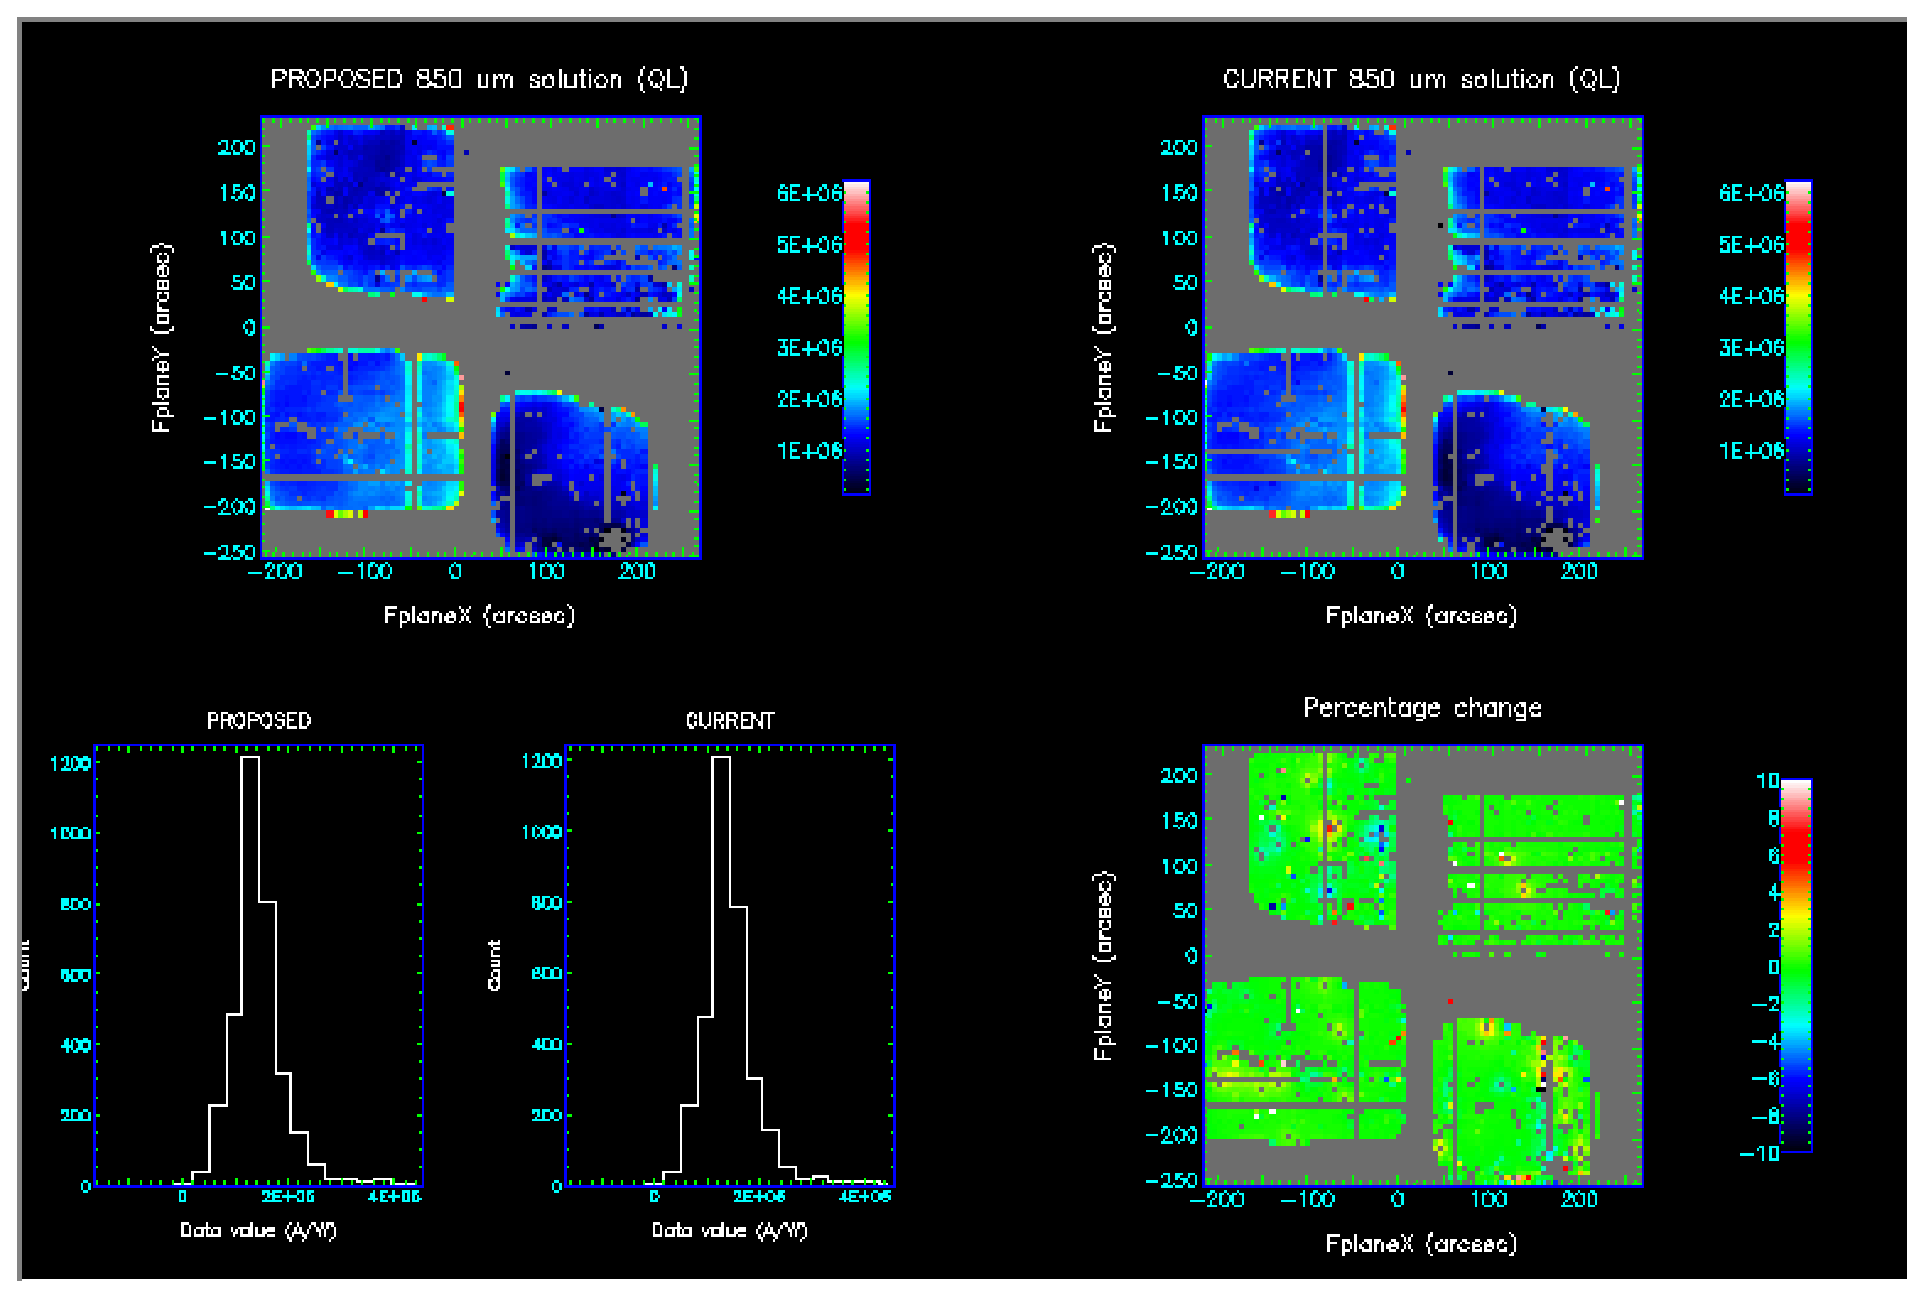
\includegraphics[width=\textwidth]{sun264_flatfield.eps}
\caption{Example display from a FLATFIELD observation or FASTFLAT
  sequence. The top left panel is the responsivity map for this
  observation (containing the proposed new solution), the top right
  panel shows the current responsivity solution (i.e\ currently in
  use) for comparison. The bottom left panels are responsivity
  histograms for this observation and the current solution (PROPOSED
  and CURRENT respectively). The bottom right panel shows the
  percentage change in the responsivities between this observation and
  the current solution in use, scaled between
  $\pm10$\,\%.\label{fig:flatfield}}
\end{figure}

Once complete, the pipeline writes a flag file in
\verb+ORAC_DATA_OUT+ for the current observation containing the name
of each successful flatfield solution. The flag file is a hidden file
with the name \verb+.sYYYYMMDD_MMMMM.ok+ where \verb+YYYYMMDD+ is the
UT date and \verb+MMMMM+ is the zero-padded observation number. This
file is used by the telescope control system (TCS) at the JCMT to
identify the new flatfields to use in subsequent observations.

\subsubsection{Fast-ramps}

The fast-ramp flatfields (FASTFLAT) taken as part of on-sky observing
are included with the science data and processed as part of
map-making, but may be processed separately using the
\task{REDUCE\_FASTFLAT} recipe to assess how much the responsivities
change during an observation. The results are calculated and displayed
as above, but in this case the second fast-ramp flatfield is compared
with the first, and not with the internal flatfield solution.

Fast-ramp flatfields are also processed separately in the QL and
summit pipelines and picked up as necessary for map-making or noise
calculations.

\subsection{NOISE}

Noise observations are a series of measurements recording the
bolometer signal either against a dark shutter or open to the
atmosphere. The telescope is not tracking a source during the
measurement. The recipe calculates the average power spectrum of each
array. The \SMURF\ task \task{calcnoise} is used to calculate the
noise properties for each subarray between 2 and 10\,Hz. The recipe
calibrates the noise data using the appropriate FCF to calculate the
noise equivalent flux density (NEFD). If the measurement is on sky,
the NEFD is also quoted for the zenith, using the current optical
depth and airmass.

A numerical summary of the noise properties, showing the mean, median
and modal noise values, the effective noise equivalent power and
number of bolometers, is written to the screen. These results are also
written to a log file called \verb+log.bolonoise+. The NEFD results
are written to a log file called \verb+log.nefd+.

Focal-plane mosaics of the noise, the percentage change in the noise
since the last measurement and the NEP are displayed in a Kapview
window along with a histogram of the noise values (see
Fig.~\ref{fig:noise}).

The QL and summit pipelines process each file as it is written to
disk. Otherwise all of the data (for a given subarray) are passed to
\task{calcnoise}.

\begin{figure}[t]
\centering
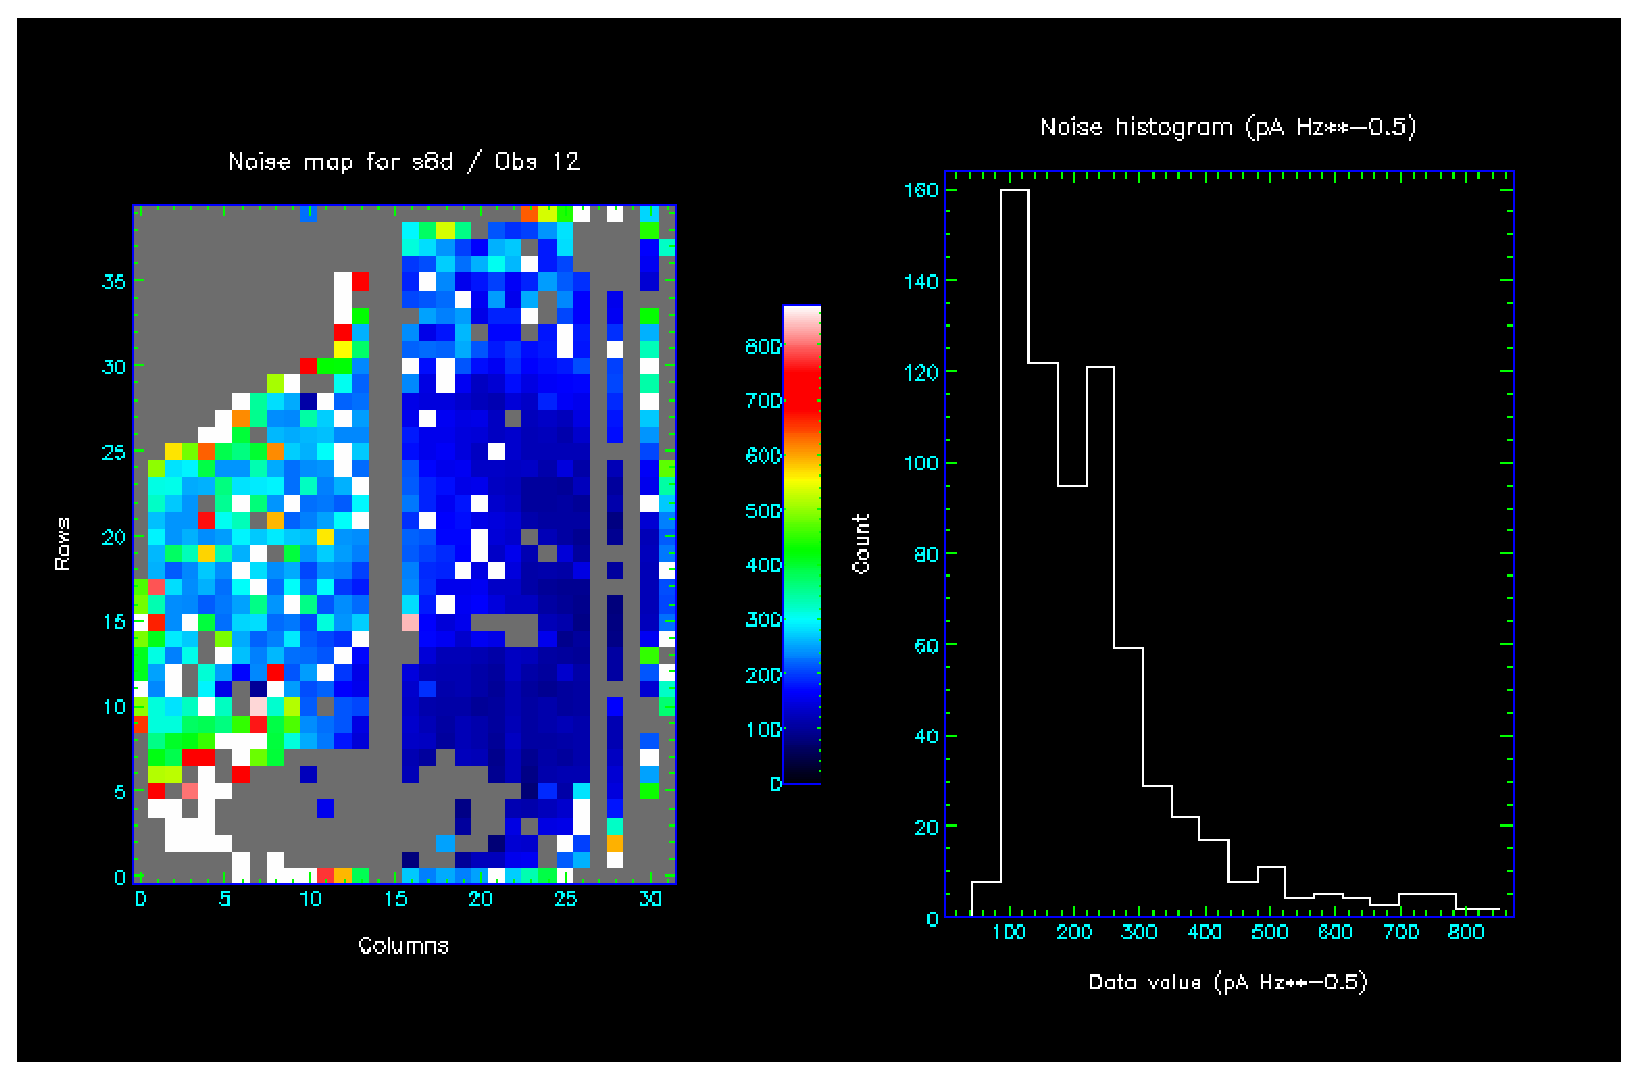
\includegraphics[width=\textwidth]{sun264_noise.eps}
\caption{Example display from a NOISE observation. The top-left panel
  displays the noise for the current data, while the top-right panel
  shows the percentage change since the previous noise
  measurement. The bottom-left panel shows a histogram of noise
  values, while the bottom-right shows the NEP for the current
  data.\label{fig:noise}}
\end{figure}

\subsection{POINTING}

Pointing observations consist of making a map of a point source, and
are processed with the \task{REDUCE\_POINTING} recipe. The recipe
processes the data with the iterative map-maker, crops the image to
75\,arcsec on a side and removes any residual large-scale background
signal with \CUPID\ \task{findback}. If the source is a known
calibrator, the pipeline derives an FCF.

The name of the processed image is written into a flag file (as for
FLATFIELD observations above). The flag file is read by the telescope
POINTING\_FOCUS task which analyzes the named image to calculate the
pointing offsets applied to the telescope pointing model.

The pipeline makes its own estimate of the pointing offsets in two
ways by applying a point-source filter (matched filter) to enhance the
signal-to-noise ratio in the image followed by fitting a 2-D profile
to the source and calculating the centroid position. Both results are
written to a log file called \verb+log.pointing+.

The pipeline displays the image used to derive the pointing offsets in
a \GAIA\ window. The recipe also fits a 2-d profile to the source and
writes the result to a log file called \verb+log.beam+.

The map-maker uses the config file \verb+dimmconfig_pointing.lis+,
except for very short pointing observations (defined as $<15$\,s)
which use \verb+dimmconfig_veryshort_planet.lis+ for planets and
\verb+dimmconfig_bright_compact_veryshort.lis+ for all other sources.

The QL pipeline uses the \task{REDUCE\_POINTING\_QL} recipe, which
contains different logic for dealing with DREAM and STARE data but is
functionally identical to the main \task{REDUCE\_POINTING} recipe for
SCAN data.

\subsection{FOCUS}

Focus observations are processed with the \task{REDUCE\_FOCUS}
recipe. A focus observation consists of a series of maps made of a
point source with the secondary mirror (SMU) at various
positions. Only one axis (eother X, Y or Z) is varied at a time.

In the QL pipeline, the maps are made as the data are taken and
collated once the observation has ended. (In practice, due to the fact
that the QL pipeline cannot rely on the \verb+OBSEND+ FITS header, an
observation is considered to have ended once an image exists at each
of the SMU positions: the number of SMU positions is retrieved from
the FITS header.) The non-QL pipeline processes each SMU setting in
turn.

Once all the maps exist, the pipeline creates a cube with the third
axis given by the SMU position. The images are registered to the same
pixel coordinates before adding to the cube so that they align
correctly.

The pipeline writes a flag file (as above) which contains the name of
the data cube. The flag file is read by the telescope POINTING\_FOCUS
task which analyzes the cube to calculate the best SMU position. The
pipeline makes its own estimate of the best-fit SMU position by
fitting a parabola to the peak fluxes derived from 2-D fits (provided
at least three fluxes could be derived) and writes that number to a
log file called \verb+log.focus+.

The images at each focus position are displayed in sequence in a
single Kapview window (see Figure \ref{fig:focus}).

\begin{figure}[t]
\centering
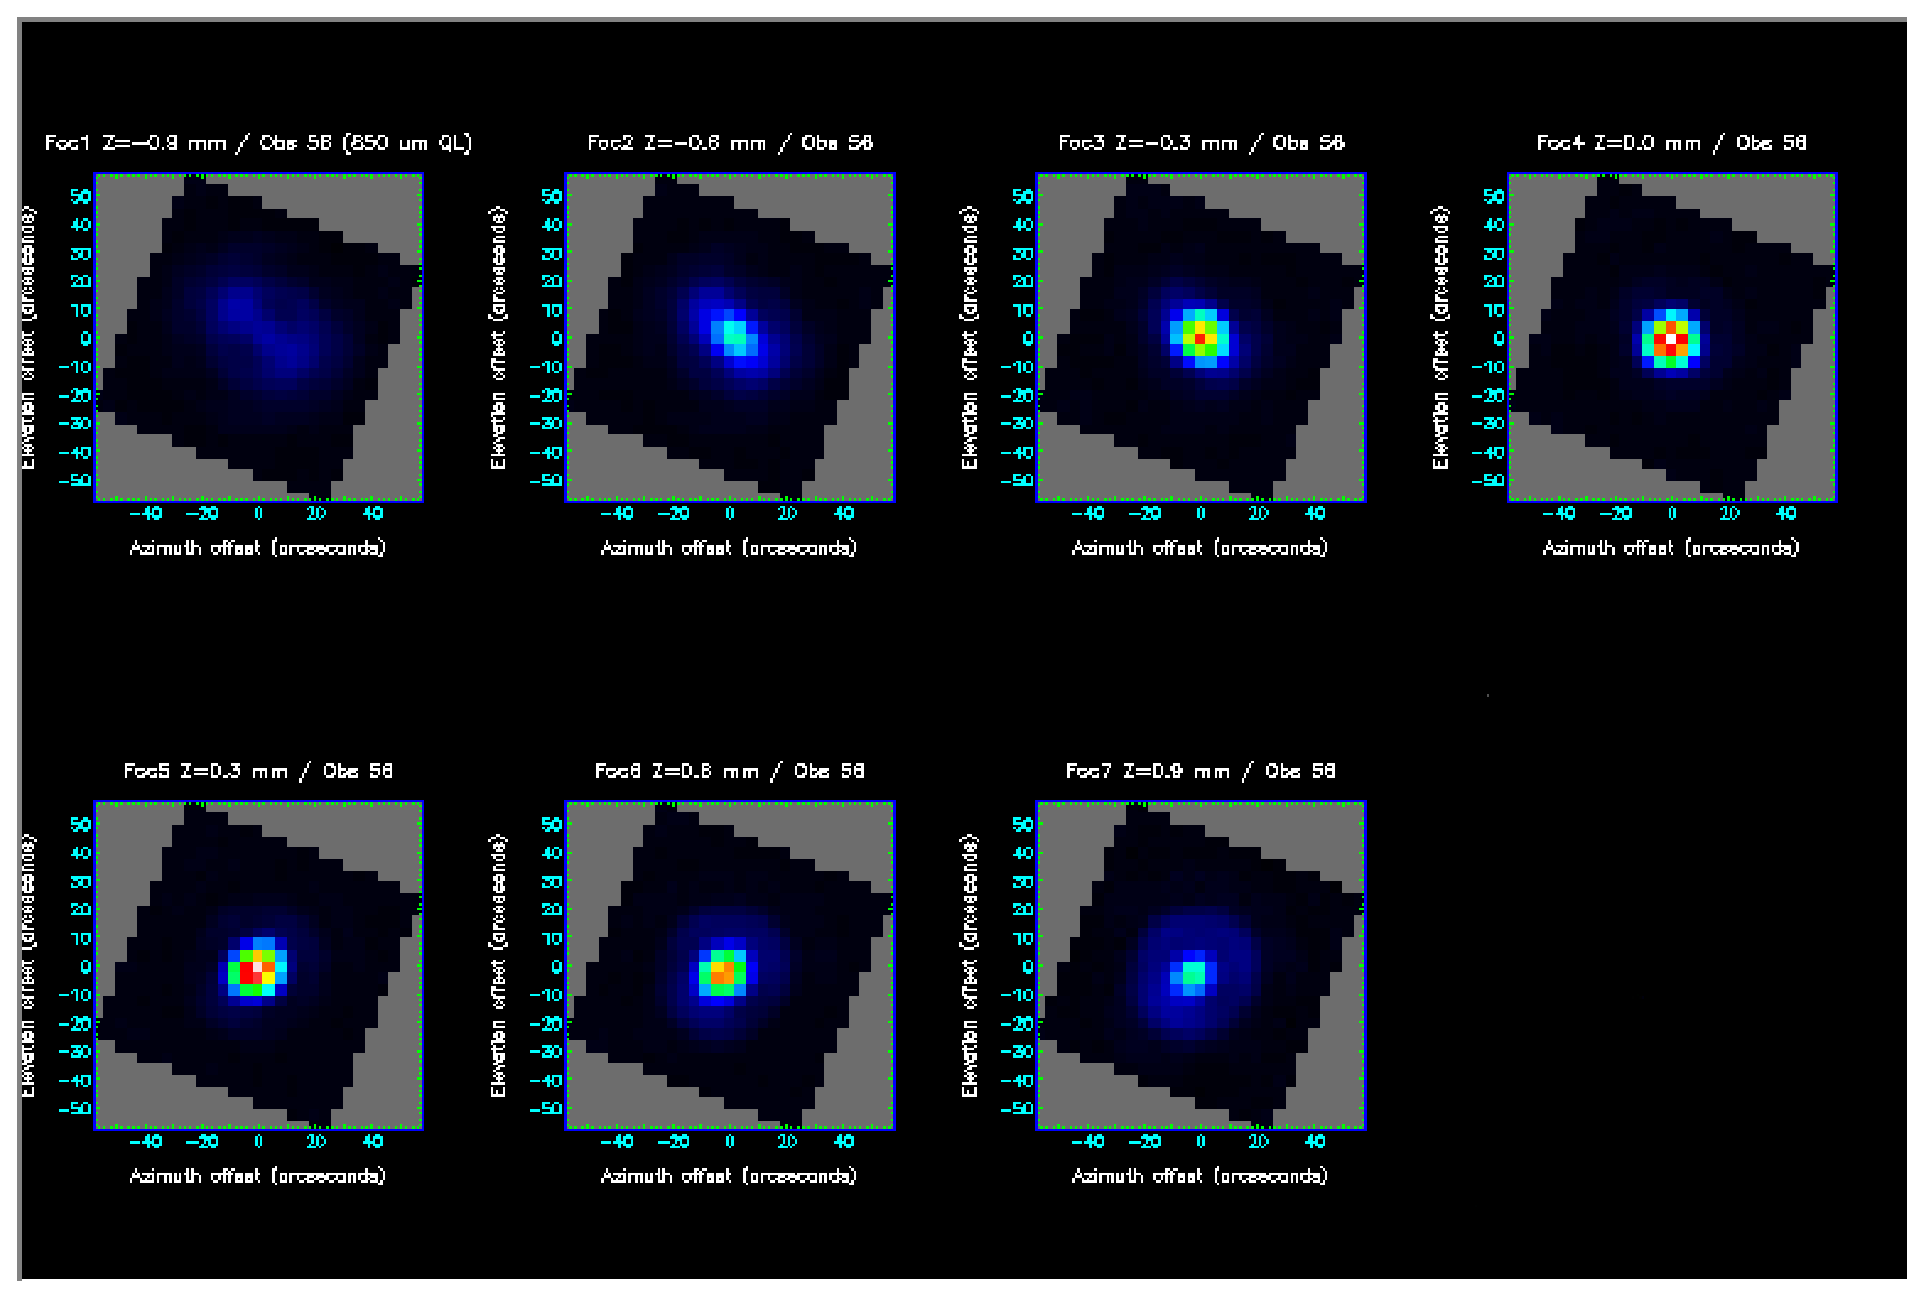
\includegraphics[width=\textwidth]{sun264_focus.eps}
\caption{Example display from a FOCUS observation showing a reduced
  image for each of seven SMU positions. The SMU position (and axis)
  is given in the title for each image. The images are displayed with
  axes of arcsecond offsets.\label{fig:focus}}
\end{figure}

The map-maker uses either the \verb+dimmconfig_veryshort_planet.lis+
for planets and \\ \verb+dimmconfig_bright_compact_veryshort.lis+ for
all other sources.

The same recipe is used for all forms of the pipeline. The output cube
has the suffix \verb+_foc+.

\subsection{SETUP}

A SETUP observation consists of a fast-ramp flatfield (FASTFLAT)
measurement followed by a NOISE, both taken with the shutter
closed. The recipe processes each separately as described for the
respective observation types above. The results of processing each
type of data are displayed in separate Kapview windows. The pipeline
writes a flag file at the end of the observation with the names of the
files containing the names of the flatfield solutions and noise
calculations for the telescope software to read.

\subsection{SKYDIP}

A SKYDIP observation is a series of NOISE-SKY observations at
differing airmass. Currently there is no pipeline recipe to process
these data, other than as a NOISE observation.


\section{\xlabel{engineering}Engineering Data\label{se:eng}}

Recipes also exist for processing engineering data, usually taken with
the shutter closed and the telescope stationary. Historically, the
real-time sequencer (RTS) was not involved in such measurements which
prevented the pipeline from processing these data due to missing FITS
headers and other essential metadata.

In September 2010 is was decided that the pipeline be used to process
and analyze data taken in engineering mode, and a simulated RTS is
used to generate metadata. Support for engineering data is currently
quite rudimentary with only a single recipe available.

Note that in order to process data taken in engineering mode, the
\verb+-eng+ option must be given to the \oracdr\ initialization
script.

\subsection{NEP}

Measurements of the noise-equivalent power (NEP) are processed with
the \task{ENG\_NEP} recipe. The `observation' consists of a series of
NOISE measurements at different pixel heater and detector bias
values. The recipe is designed to run offline, after the observation
has finished.

The NEP is calculated for each subarray at each setting. These
per-bolometer NEP images are combined to form a 4-d hypercube with
axes bolometer row, bolometer column, heater setting and bias setting
for each subarray. These hypercubes are named
\verb+sXXYYYYMMDD_MMMMM_nep.sdf+ where \verb+sXX+ is the subarray
label (e.g.\ \verb+s8a+).

From these data, the effective and RMS NEP is calculated at each
heater and bias setting, stored as a 2-d image with the heater and
bias values as the X- and Y axes. These images have suffices of
\verb+_effnep+ and \verb+_rmsnep+ respectively.

A number of log files are also written. The first is called
\verb+log.bolonoise+ which contains the noise properties for each
heater and bias setting and all subarrays. Log files for the `mapping
speed' parameter for each subarray are written separately with the
name \verb+log.mapspeed_SXX+ where \verb+SXX+ is the subarray
(e.g.\ s4a). The mapping speed is given by $N_{\rm bol} / {\rm
  NEP}_{\rm RMS}^2$ and is calculated for the best $N_{\rm bol}$
bolometers between 300 and 1000 in steps of 100 bolometers.

The recipe does not display any data.

\section{\xlabel{dataproducts}Data products (output files)\label{se:dataprod}}

The output maps from the pipeline are Starlink NDF files with a number
of NDF components, which may be listed with \task{hdstrace}. The
full hierarchy is shown in the example trace below.

The files contain standard the DATA and VARIANCE components. Images
have a three-dimensional WCS added, namely RA-Dec-wavelength. The
third axis is a single-pixel wide and is wavelength in m (sometimes
referred to as a non-significant axis, on the basis that it is not
always necessary to specify it). A FITS header extension is written
with values collated from all the files that went in to producing the
image. The FITS extension may be viewed with
\KAPPA\ \task{fitslist}. The UNITS component contains the current units
of the file, usually mJy\,beam$^{-1}$, along with the LABEL (a text
description of the units). The source name is written into the TITLE
field.

\SMURF\ \task{makemap} also writes additional NDF extensions under the
\verb+.MORE.SMURF+ hierarchy called \verb+EXP_TIME+ and
\verb+WEIGHTS+. The former is the exposure time image, the latter is
the number of `hits' on a given pixel (i.e.\ the number of
measurements that went into that pixel). Each of these NDFs has its
own WCS, UNITS and LABEL.

\KAPPA\ \task{hislist} will print the HISTORY embedded in the file,
which also shows the full list of arguments to \task{makemap}. The
PROVENANCE my be examined with \KAPPA\ \task{provshow}.

Example trace:
\begin{myquote}
\begin{verbatim}
GS20091205_22_8  <NDF>

   DATA_ARRAY     <ARRAY>         {structure}
      DATA(990,1036,1)  <_DOUBLE>    *,*,*,*,*,*,*,*,*,*,*,*,*,*,*,*,*,*,
                                     *,*,*,*,*,*,*,*,*,*,*,*,*,*,*,*,*,*,*
      ORIGIN(3)      <_INTEGER>      -494,-522,1

   TITLE          <_CHAR*3>       'W5E'
   LABEL          <_CHAR*12>      'Flux Density'
   UNITS          <_CHAR*8>       'mJy/beam'
   VARIANCE       <ARRAY>         {structure}
      DATA(990,1036,1)  <_DOUBLE>    *,*,*,*,*,*,*,*,*,*,*,*,*,*,*,*,*,*,
                                     *,*,*,*,*,*,*,*,*,*,*,*,*,*,*,*,*,*,*
      ORIGIN(3)      <_INTEGER>      -494,-522,1

   WCS            <WCS>           {structure}
      DATA(221)      <_CHAR*32>      ' Begin FrameSet',' Nframe = 5',' Cu...'
                                     ... ' E...',' End CmpMap',' End
FrameSet'

   HISTORY        <HISTORY>       {structure}
      CREATED        <_CHAR*24>      '2011-JAN-10 21:41:27.349'
      CURRENT_RECORD  <_INTEGER>     12
      RECORDS(15)    <HIST_REC>      {array of structures}

      Contents of RECORDS(1)
         DATE           <_CHAR*24>      '2011-JAN-10 21:41:28.417'
         COMMAND        <_CHAR*30>      'MAKEMAP         (SMURF V1.1.0)'
         USER           <_CHAR*5>       'agibb'
         HOST           <_CHAR*7>       'aspersa'
         DATASET        <_CHAR*77>
'/scuba2/jcmtdata/reduced/scuba2_8...'
         TEXT(70)       <_CHAR*72>      'Parameters: ALIGNSYS=FALSE BBM=',
                                        ... '   s8d20091205_00022_0042,
s8...'

   MORE           <EXT>           {structure}
      SMURF          <SMURF_EXT>     {structure}
         WEIGHTS        <NDF>           {structure}
            DATA_ARRAY     <ARRAY>         {structure}
               DATA(990,1036)  <_DOUBLE>      *,*,*,*,*,*,*,*,*,*,*,*,*,*,
                                              *,*,*,*,*,*,*,*,*,*,*,*,*,*
               ORIGIN(2)      <_INTEGER>      -494,-522

            LABEL          <_CHAR*6>       'Weight'
            WCS            <WCS>           {structure}
               DATA(175)      <_CHAR*32>      ' Begin FrameSet',' Nframe =
5',
                                              ... ' End Cm...',' End
FrameSet'

            UNITS          <_CHAR*6>       'pW**-2'

         EXP_TIME       <NDF>           {structure}
            DATA_ARRAY     <ARRAY>         {structure}
               DATA(990,1036)  <_DOUBLE>      *,*,*,*,*,*,*,*,*,*,*,*,*,*,
                                              *,*,*,*,*,*,*,*,*,*,*,*,*,*
               ORIGIN(2)      <_INTEGER>      -494,-522

            LABEL          <_CHAR*19>      'Total exposure time'
            UNITS          <_CHAR*1>       's'
            WCS            <WCS>           {structure}
               DATA(175)      <_CHAR*32>      ' Begin FrameSet',' Nframe =
5',
                                              ... ' End Cm...',' End
FrameSet'

      PROVENANCE     <PROVENANCE>    {structure}
         ANCESTORS(45)  <PROV>          {array of structures}

         Contents of ANCESTORS(1)
            PATH           <_CHAR*74>
'/scuba2/jcmtdata/reduced/scuba...'
            DATE           <_CHAR*19>      '2011-01-10 21:48:49'
            CREATOR        <_CHAR*13>      'KAPPA:NDFCOPY'
            HISTORY(1)     <HISREC>        {structure}
               DATE           <_CHAR*24>      '2011-JAN-10 21:49:14.648'
               COMMAND        <_CHAR*30>      'NDFCOPY         (KAPPA
1.12-4)'
               USER           <_CHAR*5>       'agibb'
               TEXT           <_CHAR*228>     'Parameters: COMP='DATA'
EXT...'

            PARENTS(1)     <_INTEGER>      2

         DATE           <_CHAR*19>      '2011-01-10 21:48:49'
         CREATOR        <_CHAR*13>      'KAPPA:NDFCOPY'
         HASH           <_INTEGER>      789255632
         PARENTS(1)     <_INTEGER>      1

      FITS(201)      <_CHAR*80>      'TELESCOP= 'JCMT    '           / Na...'
                                     ... 'NBOLOEFF=     529.152083333333
/...'

End of Trace.
\end{verbatim}
\end{myquote}

\subsection{Log files}

The pipeline writes out a number of log files with the results of
various calculations made during the data reduction. The main science
recipe produces log files for the image noise and the noise-equivalent
flux density (NEFD), called \texttt{log.noise} and \texttt{log.nefd}
respectively. Both values are calculated for the individual
observation images and the final coadd. The noise is calculated as the
median error value (i.e.\ square-root of the variance) and given in
mJy\,beam$^{-1}$. The NEFD is calculated from the square-root of the
product of the variance and the exposure time NDF components, and the
median value taken as the representative NEFD (in mJy\,$\sqrt{\rm s}$).

\section{\xlabel{picard}Analysis of processed data\label{picard}}

A variety of simple \picard\ recipes (see \picardsun) exist to perform
post-processing analysis.

SCUBA-2 specific \picard\ recipes begin with or contain the word
\verb+SCUBA2+; recipes specific to processing JCMT data contain
\verb+JCMT+. Documentation for each recipe is given in \picardsun, and
on the \picard\ home page,
\htmladdnormallink{\texttt{http://www.oracdr.org/oracdr/PICARD}}{http://www.oracdr.org/oracdr/PICARD}
where each recipe is fully documented.

Running \picard\ is simple. For example:
\begin{myquote}
\begin{verbatim}
% picard -recpars <recipe_param_file> RECIPE <list_of_files>
\end{verbatim}
\end{myquote}
where \verb+<recipe_param_file>+ is a text file containing the
relevant recipe parameters, \verb+RECIPE+ is the name of the
recipe to run and \verb+<list_of_files>+ is the list of NDF files to
process, which must exist in the current directory. The output files
are written to the current directory, or the directory defined by
\verb+ORAC_DATA_OUT+.

Most recipes have one or more recipe parameters which can be specified
using the \texttt{-recpars} option. Recipe parameters are given in a
text file with the following format:
\begin{myquote}
\begin{verbatim}
[RECIPE_NAME]
RECIPE_PARAMETER1 = value1
RECIPE_PARAMETER2 = value2
\end{verbatim}
\end{myquote}
The available recipe parameters are listed in the documentation on the
\picard\ home page above and in \picardsun.

The recommended approach for a few common tasks is detailed below.

\subsection{Coadding/mosaicking multiple images}

Although the pipeline will mosaic observations of the same target from
the same night, it is clearly desirable to combine data from multiple
nights. Alternatively, the user may wish to exert some additional
control over the mosaicking parameters.

The \task{MOSAIC\_JCMT\_IMAGES} recipe deals with processed JCMT data
(including ACSIS data cubes) and takes into account the
instrument-specific NDF components such as the exposure time
(\verb+EXP_TIME+ -- see \S\ \ref{se:dataprod} above). The choice of
coadding task is left to the user and may be either
\CCDPACK\ \task{makemos} or \KAPPA\ \task{wcsmosaic} (the default). If
using \task{makemos}, images are first aligned using
\KAPPA\ \task{wcsalign}. By default, the images (and additional NDF
components) are combined using a nearest-neighbour scheme but this may
be overridden by specifying the relevant parameter for
\task{wcsmosaic} or \task{wcsalign}.

For images which contain a bright source, there is also the option to
register the images to a common centre (see \S\ \ref{se:reg}
below). If chosen, the user must provide the coordinates (equatorial
in sexagesimal format, i.e.\ \verb+HH:MM:SS.S, DD:MM:SS.S+) of that
source, unless it is a known calibrator (in which case the WCS
reference position will be used instead). Note that choosing this
option will modify the WCS of the input files. If this is not desired,
the user should register the images separately using the recipe
\task{SCUBA2\_REGISTER\_IMAGES} (see \S\ \ref{se:reg} below).

The output mosaic takes its name from the last input file in the list
and has the suffix \verb+_mos+. The user should take care to ensure
this file does not already exist otherwise it will be overwritten.

\subsection{Registering images to a common centre\label{se:reg}}

Random pointing offsets and drifts between observations on a given
night (and over different nights) mean that the final mosaic of a
point source will not be optimal, and any faint surrounding structure
may be masked entirely.

The recipe \task{SCUBA2\_REGISTER\_IMAGES} is specific to SCUBA-2
data.  The approach is to find the position of a given source in each
image and apply a shift to the WCS so that the peak fitted positions
are coincident for each image.

Several recipe parameters are required, namely the coordinates of the
reference position. Currently only equatorial coordinates are
supported and must be written in sexagesimal format. The registered
images have the suffix \verb+_reg+.

As with the mosaicking recipe, this recipe knows about and takes care
of applying the same shift to the \verb+EXP_TIME+ and \verb+WEIGHTS+
components, so the combined results are accurate.


\newpage
\appendix
\section{\xlabel{ap_list}Alphabetical list of SCUBA-2 recipes\label{ap:list}}
\begin{htmlonly}
\begin{description}
\end{htmlonly}
\menuitem{ARRAY\_TESTS}{
  Co-add and display DREAM/STARE images}
\menuitem{ASSESS\_DATA\_NOISE}{
  Calculate noise properties of SCUBA-2 data}
\menuitem{BENCHMARK}{
  Benchmarking recipe}
\menuitem{ENG\_NEP}{
  Process NEP measurements made in engineering mode}
\menuitem{ENG\_NEP\_QL}{
  QL processing NEP measurements made in engineering mode}
\menuitem{REDUCE\_DARK}{
  Process dark frames}
\menuitem{REDUCE\_DREAMSTARE}{
  Process DREAM/STARE images}
\menuitem{REDUCE\_DREAMSTARE\_QL}{
  QL processing DREAM/STARE images}
\menuitem{REDUCE\_FASTFLAT}{
  Process fast-ramp flatfield data}
\menuitem{REDUCE\_FLATFIELD}{
  Process flatfield measurements}
\menuitem{REDUCE\_FOCUS}{
  Recipe for deriving focus information}
\menuitem{REDUCE\_FOCUS\_QL}{
  process focus observations in the quick-look pipeline}
\menuitem{REDUCE\_FOCUS\_SUMMIT}{
  derive focus information in the summit pipeline}
\menuitem{REDUCE\_FTS\_FOCUS}{
  Recipe for processing FTS-2 focus observations}
\menuitem{REDUCE\_FTS\_POINTING}{
  Recipe for processing FTS-2 pointing observations}
\menuitem{REDUCE\_FTS\_SCAN}{
  Recipe for processing FTS-2 SCAN data}
\menuitem{REDUCE\_FTS\_ZPD}{
  Recipe for processing FTS-2 SCAN data}
\menuitem{REDUCE\_NOISE}{
  Process NOISE observations}
\menuitem{REDUCE\_NOISE\_PHOTON}{
  determine photon noise contribution to total noise}
\menuitem{REDUCE\_NOISE\_QL}{
  QL processing NOISE observations}
\menuitem{REDUCE\_NOISE\_SUMMIT}{
  Summit processing NOISE observations}
\menuitem{REDUCE\_POINTING}{
  Process POINTING observations}
\menuitem{REDUCE\_POINTING\_QL}{
  QL processing of POINTING observations}
\menuitem{REDUCE\_POINTING\_SUMMIT}{
  Process POINTING observations in the summit pipeline}
\menuitem{REDUCE\_POL\_STARE}{
  Recipe for processing POL-2 stare data}
\menuitem{REDUCE\_SASSY}{
  Process data for the SASSy project}
\menuitem{REDUCE\_SCAN}{
  Process SCAN-mode data}
\menuitem{REDUCE\_SCAN\_EXTENDED\_SOURCES}{
  Process SCAN data from extended sources}
\menuitem{REDUCE\_SCAN\_FAINT\_POINT\_SOURCES}{
  Process SCAN data from faint compact sources}
\menuitem{REDUCE\_SCAN\_FAINT\_POINT\_SOURCES\_JACKKNIFE}{
  Process blank field data with a jack-knife-based method}
\menuitem{REDUCE\_SCAN\_FAKEMAP}{
  Process SCAN data with existing map data added}
\menuitem{REDUCE\_SCAN\_QL}{
  QL process SCAN data}
\menuitem{REDUCE\_SCAN\_SUMMIT}{
  Summit recipe for processing SCAN data}
\menuitem{REDUCE\_SETUP}{
  process data from a setup observation}
\menuitem{REDUCE\_SETUP\_QL}{
  process data from a setup observation in the QL pipeline}
\menuitem{REDUCE\_SETUP\_SUMMIT}{
  process data from a setup observation in the summit pipeline}
\menuitem{REDUCE\_SKYDIP}{
  Process SKYDIP observations}
\menuitem{REDUCE\_SKYDIP\_QL}{
  Process SKYDIP observations with the quick-look pipeline}
\menuitem{REDUCE\_SKYDIP\_SUMMIT}{
  Process SKYDIP observations with the summit pipeline}
\begin{htmlonly}
\end{description}
\end{htmlonly}

\newpage
\begin{small}
\section{\xlabel{ap_classified}Classified list of SCUBA-2 recipes\label{ap:classified}}

SCUBA-2 recipes may be classified in terms of their observing mode as
follows.

{\large
\begin{center}
{\bf Science data: SCAN mode}
\end{center}
}

\begin{description}
\classitem{REDUCE\_CLS}
Process data taken as part of the Cosmology Legacy Survey
\classitem{REDUCE\_SASSY}
Process data for the SASSy project
\classitem{REDUCE\_SCAN}
Process SCAN-mode data
\classitem{REDUCE\_SCAN\_EXTENDED\_SOURCES}
Process SCAN data from extended sources
\classitem{REDUCE\_SCAN\_FAINT\_POINT\_SOURCES}
Process SCAN data from faint compact sources
\classitem{REDUCE\_SCAN\_FAINT\_POINT\_SOURCES\_JACKKNIFE}
Process blank field data with a jack-knife-based method
\classitem{REDUCE\_SCAN\_FAKEMAP}
Process SCAN data with existing map data added
\classitem{REDUCE\_SCAN\_QL}
QL process SCAN data
\classitem{REDUCE\_SCAN\_SUMMIT}
Summit recipe for processing SCAN data
\end{description}

{\large
\begin{center}
{\bf Science data: DREAM/STARE mode}
\end{center}
}
\begin{description}
\classitem{REDUCE\_DREAMSTARE}
Process DREAM/STARE images
\classitem{REDUCE\_DREAMSTARE\_QL}
QL processing DREAM/STARE images
\end{description}

{\large
\begin{center}
{\bf Science data: FTS-2}
\end{center}
}
\begin{description}
\classitem{REDUCE\_FTS\_FOCUS}
Recipe for processing FTS-2 focus observations
\classitem{REDUCE\_FTS\_POINTING}
Recipe for processing FTS-2 pointing observations
\classitem{REDUCE\_FTS\_SCAN}
Recipe for processing FTS-2 SCAN data
\classitem{REDUCE\_FTS\_ZPD}
Recipe for processing FTS-2 SCAN data
\end{description}

{\large
\begin{center}
{\bf Science data: POL-2}
\end{center}
}
\begin{description}
\classitem{REDUCE\_POL\_STARE}
Recipe for processing POL-2 stare data
\end{description}

{\large
\begin{center}
{\bf Pointing observations}
\end{center}
}
\begin{description}
\classitem{REDUCE\_POINTING}
Process POINTING observations
\classitem{REDUCE\_POINTING\_QL}
QL processing of pointing observations
\classitem{REDUCE\_POINTING\_SUMMIT}
Summit processing of pointing observations
\end{description}

{\large
\begin{center}
{\bf Focus observations}
\end{center}
}
\begin{description}
\classitem{REDUCE\_FOCUS}
Recipe for deriving focus information
\classitem{REDUCE\_FOCUS\_QL}
process focus observations in the quick-look pipeline
\classitem{REDUCE\_FOCUS\_SUMMIT}
derive focus information in the summit pipeline
\end{description}

{\large
\begin{center}
{\bf Noise observations}
\end{center}
}
\begin{description}
\classitem{ASSESS\_DATA\_NOISE}
Calculate noise properties of SCUBA-2 data
\classitem{ENG\_NEP}
Process NEP measurements made in engineering mode
\classitem{REDUCE\_NOISE}
Process NOISE observations
\classitem{REDUCE\_NOISE\_PHOTON}
determine photon noise contribution to total noise
\classitem{REDUCE\_NOISE\_QL}
QL processing NOISE observations
\classitem{REDUCE\_SKYDIP}
Process SKYDIP observations
\end{description}

{\large
\begin{center}
{\bf Flatfield observations}
\end{center}
}
\begin{description}
\classitem{REDUCE\_FASTFLAT}
Process fast-ramp flatfield data
\classitem{REDUCE\_FLATFIELD}
Process flatfield measurements
\end{description}

{\large
\begin{center}
{\bf Setup observations}
\end{center}
}
\begin{description}
\classitem{REDUCE\_SETUP}
process data from a setup observation
\classitem{REDUCE\_SETUP\_QL}
process data from a setup observation in the QL pipeline
\classitem{REDUCE\_SETUP\_SUMMIT}
process data from a setup observation in the summit pipeline
\end{description}

{\large
\begin{center}
{\bf QL-pipeline recipes}
\end{center}
}
\begin{description}
\classitem{REDUCE\_DREAMSTARE\_QL}
QL processing DREAM/STARE images
\classitem{REDUCE\_FOCUS\_QL}
process focus observations in the quick-look pipeline
\classitem{REDUCE\_NOISE\_QL}
QL processing NOISE observations
\classitem{REDUCE\_POINTING\_QL}
QL processing of pointing observations
\classitem{REDUCE\_SCAN\_QL}
QL process SCAN data
\classitem{REDUCE\_SETUP\_QL}
process data from a setup observation in the QL pipeline
\end{description}

{\large
\begin{center}
{\bf Summit-pipeline recipes}
\end{center}
}
\begin{description}
\classitem{REDUCE\_FOCUS\_SUMMIT}
derive focus information in the summit pipeline
\classitem{REDUCE\_POINTING\_SUMMIT}
Summit processing of pointing observations
\classitem{REDUCE\_SCAN\_SUMMIT}
Summit recipe for processing SCAN data
\classitem{REDUCE\_SETUP\_SUMMIT}
process data from a setup observation in the summit pipeline
\classitem{REDUCE\_SKYDIP\_SUMMIT}
Process SKYDIP observations with the summit pipeline
\end{description}

{\large
\begin{center}
{\bf Miscellaneous}
\end{center}
}
\begin{description}
\classitem{ARRAY\_TESTS}
Co-add and display DREAM/STARE images
\classitem{BENCHMARK}
Benchmarking recipe
\classitem{REDUCE\_DARK}
Process dark frames
\end{description}


\end{small}
\newpage

\section{\xlabel{ap_full}Specifications of SCUBA-2 recipes\label{ap:full}}

The following pages describe the SCUBA-2 recipes in detail.

\newpage
\newpage
\sstroutine{
   ARRAY\_TESTS
}{
   Co-add and display DREAM/STARE images
}{
   \sstdescription{
      Basic processing recipe suitable for DREAM/STARE images from a
      single subarray. This recipe is designed to be used for
      lab-testing only.

      No alignment is done on the images so that they are mosaicked in
      the pixel frame (this means that if data exists from multiple
      subarrays, they will be averaged together!). A method to determine
      the frame-to-frame variance is provided which writes out to a log
      file called log.noise which can be monitored by the StripChart.
      The relevant column to monitor is {\tt "}noise{\tt "}.
   }
   \sstnotes{
      \sstitemlist{

         \sstitem
         This primitive is not designed to handle time series observing
         modes.

         \sstitem
         If the frames are identical, then the Group mosaicked image
         with contain {\tt "}NaN{\tt "}. In that case, add the argument GENVAR=0 to
         \_MAKE\_MOSAIC\_FRAME\_.

         \sstitem
         If there is no variance, {\tt "}NaN{\tt "} will be written to log.noise.
         The stripchart may or may not do something sensible with that.

         \sstitem
         The Group image variance is written to log.noise for monitoring
         with the StripChart.
      }
   }
   \sstdiytopic{
      Display
   }{
      The Frame image is displayed in Gaia window 1.
      The Group image is displayed in Gaia window 2; its variance is
      displayed in window 3.
   }
}
\newpage
\sstroutine{
   ASSESS\_DATA\_NOISE
}{
   Calculate noise properties of SCUBA-2 data
}{
   \sstdescription{
      This recipe is designed to provide observers with a simple
      assessment of the noise properties of their data. It does this by
      calculating the noise for either the first on-sky data file
      (default) or for the entire time stream. The results are passed
      through the same quality assurance (QA) checks as performed by the
      quick-look (QL) pipeline running at the telescope.

      The processing is controlled by the recipe parameters described
      below.
   }
   \sstnotes{
      None.
   }
   \sstdiylist{
      Available Parameters
   }{
      \sstsubsection{
         The following recipe parameters can be set via the --recpars
      }{
      }
      \sstsubsection{
         option:
      }{
      }
      \sstsubsection{
         NOISE\_CALC
      }{
         Type of noise calculation to perform. May be full, which
         calculates the noise properties of the entire time stream or
         quick to use only the first on-sky subscan (30 seconds).
      }
      \sstsubsection{
         NOISE\_CFG
      }{
         The name of a config file to use when calculating the noise
         properties. The default is to use the standard noise config but
         the user is advised to supply the same config used in the
         map-making process.
      }
      \sstsubsection{
         NOISE\_FREQLO
      }{
         The frequency at which to calculate the low-frequency noise.
         Default is 0.5 Hz.
      }
      \sstsubsection{
         NOISE\_FREQRANGE
      }{
         A pair of numbers indicating the frequency range (in Hz) over
         which the noise is to be calculated. Default is 2,10.
      }
   }
   \sstdiytopic{
      Display
   }{
      The focal-plane mosaic for the noise and NEP are displayed, scaled
      between 0 and the relevant spec defined by the quality assurance
      parameters. A histogram of noise values is also plotted, with the
      same upper bound.
   }
}
\newpage
\sstroutine{
   BENCHMARK
}{
   Benchmarking recipe
}{
   \sstdescription{
      Simple but realistic recipe suitable for benchmarking tests.
      Processes DREAM/STARE images. The quantity of data should always
      be the same so as to obtain meaningful comparisons.

      No images are displayed. This is purely a timing test for
      processing a standard quantity of data.
   }
   \sstnotes{
      \sstitemlist{

         \sstitem
         This recipe was originally written to process DREAM/STARE
         images but has not been updated to handle time series data. Its
         use is not recommended.
      }
   }
   \sstdiytopic{
      Display
   }{
      None.
   }
}
\newpage
\sstroutine{
   ENG\_NEP
}{
   Process NEP measurements made in engineering mode
}{
   \sstdescription{
      This recipe processes NOISE observations taken at various settings
      for the pixel heater and detector bias. The noise properties are
      calculated over a given frequency range and the resulting
      noise-equivalent power (NEP) data for each subarray are combined
      into a 4-d hypercube of the NEP as a function of bolometer
      position, heater and detector bias value.

      In addition the effective and weighted NEPs are calculated for
      each subarray and heater/bias setting.

      Details are written to log files: the noise properties are written
      to log.bolonoise as for regular noise observations, while the NEPs
      are written to log.effnep and log.wtnep.
   }
   \sstnotes{
      \sstitemlist{

         \sstitem
         Not designed to run in real time.

         \sstitem
         Bias ramp data are ignored.
      }
   }
   \sstdiylist{
      Available Parameters
   }{
      \sstsubsection{
         The following parameters can be set via the -recpars option:
      }{
      }
      \sstsubsection{
         NEP\_MAX
      }{
         Maximum NEP to be used in calculating the NEP images (W
         Hz$*$$*$-0.5). Default is 2.0e-14 W Hz$*$$*$-0.5.
      }
      \sstsubsection{
         NEP\_MIN
      }{
         Minimum NEP to be used in calculating the NEP images (W
         Hz$*$$*$-0.5). Default is 2.0e-17 W Hz$*$$*$-0.5.
      }
      \sstsubsection{
         NOISE\_FREQRANGE
      }{
         A pair of comma-separated values indicating the lower and upper
         frequency bounds (in Hz) to be used in the calculation of the
         noise properties. Default is 2,10 Hz.
      }
   }
   \sstdiytopic{
      Display
   }{
      No images are displayed.
   }
}
\newpage
\sstroutine{
   ENG\_NEP\_QL
}{
   QL processing NEP measurements made in engineering mode
}{
   \sstdescription{
      This recipe calculates the effective noise-equivalent power (NEP)
      for each subarray for a range of pixel heater and bias values. The
      results are written as an image with heater values along the
      x-axis and bias values along the y-axis.
   }
   \sstnotes{
      \sstitemlist{

         \sstitem
         Bias ramp data are ignored.

         \sstitem
         This recipe is not up to date and should not be used at this
         stage.
      }
   }
   \sstdiytopic{
      Display
   }{
      Each image is displayed in a single KAPVIEW window.
   }
}
\newpage
\sstroutine{
   REDUCE\_SCAN\_FAINT\_POINT\_SOURCES
}{
   Process SCAN data from faint compact sources
}{
   \sstdescription{
      This is the recipe for processing SCAN data for faint compact
      sources. The makemap configuration file is tuned to best deal with
      such data, though the user may specify their own.

      Raw data are passed to the map maker which are processed using the
      blank\_field config file to produce an image, which is calibrated
      in mJy/beam, displayed and tagged as a reduced product. The noise
      is estimated and the NEFD is calculated. Once all the individual
      observations have been processed, a coadd is created and
      displayed. This image is processed with a matched filter to
      enhance the signal-to-noise ratio of point sources. This image is
      tagged as a reduced product. The noise properties and NEFD for the
      new Group image are calculated and written to log files. A
      signal-to-noise ratio image is created from the matched-filtered
      image.

      Finally, the CUPID task findclumps is run using the fellwalker
      algorithm to create a source catalogue.
   }
   \sstnotes{
      \sstitemlist{

         \sstitem
         If given data from multiple sources, each source will be
         processed in full in turn.

         \sstitem
         The noise level and NEFD are stored in log.noise and log.nefd
         respectively. The noise and NEFD are calculated for each image as
         well as for the final coadd (after processing with the matched
         filter).

         \sstitem
         For large amounts of data this recipe will spend a long time
         not updating the ORAC-DR window. Check to see that makemap is
         still processing by running top or ps. (Running with -log sf is
         recommended.)

         \sstitem
         Alternative configuration parameters for the iterative
         map-maker may be specified using the recipe parameters outlined
         below.

         \sstitem
         To reduce the chance of spurious source detections, the group
         coadd is trimmed to the map size specified in the FITS header
         before running the source finder. This may not work as intended if
         the coadd contains maps with different centres.

         \sstitem
         The output catalogue, if created will have the extension .FIT.
         A clump file with suffix \_clmp will also be created.

         \sstitem
         This recipe can handle data from multiple sources and will
         correctly coadd maps, taking into account the EXP\_TIME and WEIGHTS
         components.

         \sstitem
         This recipe may be called via the shorter name
         FAINT\_POINT\_SOURCES.
      }
   }
   \sstdiylist{
      Available Parameters
   }{
      \sstsubsection{
         The following parameters can be set via the --recpars option:
      }{
      }
      \sstsubsection{
         FINDCLUMPS\_CFG
      }{
         Name of a config file for use with the CUPID findclumps task.
         The file must exist in the current working directory,
         \$FINDCLUMPS\_CONFIG\_DIR or \$ORAC\_DATA\_OUT.
      }
      \sstsubsection{
         MAKEMAP\_CONFIG
      }{
         Name of a config file for use with the SMURF makemap task. The
         file must exist in the current working directory,
         \$MAKEMAP\_CONFIG\_DIR, \$ORAC\_DATA\_OUT, \$ORAC\_DATA\_CAL or
         \$STARLINK\_DIR/share/smurf.
      }
      \sstsubsection{
         MAKEMAP\_PIXSIZE
      }{
         Size of the pixels in the output map. If not specified, the
         recipe uses the appropriate default value. Note that the
         timeseries will be downsampled to match this scale during the
         map-making process.
      }
      \sstsubsection{
         MAKEMAP\_REF
      }{
         Name of a reference image (NDF format) to use to define the
         output pixel grid. The NDF can be either 2D or 3D and the
         spatial WCS frame will be extracted.
      }
   }
   \sstdiytopic{
      Display
   }{
      The Frame image is displayed in Gaia window 1.
      The Group image is displayed in Gaia window 2; its variance is
      displayed in window 3.
   }
}
\newpage
\sstroutine{
   REDUCE\_SCAN\_FAINT\_POINT\_SOURCES\_JACKKNIFE
}{
   Process blank field data with a jack-knife-based method
}{
   \sstdescription{
      This recipe processed SCAN data and uses a jack-knife method to
      remove residual low-spatial frequency noise and create an optimal
      matched-filtered output map. The recipe proceeds as follows:

      \sstitemlist{

         \sstitem
         Each observation is processed twice using the specified
         parameters, the second time with an artificial point source added
         to the timeseries, to create a signal map and an effective PSF
         image.

         \sstitem
         These images are coadded (like with like) to produce a total
         signal map and a total effective PSF image. The amplitude of the
         source in the effective PSF image is compared with the input value
         to assess the effect the map-making process has on a point source.
         This ratio is used to scale the FCF later when calibrating the
         data.

         \sstitem
         The observations are divided into two groups which are coadded
         separately. These coadds are subtracted from one another to create
         the jack-knife map.

         \sstitem
         The angular power spectrum of the jack-knife map (which should
         consist purely of noise) is calculated and used to remove residual
         low-spatial frequency noise from the signal map and the effective
         PSF. This is the so-called whitening step (because it produces a
         map which has a noise power spectrum that is white).

         \sstitem
         The data are calibrated in mJy/beam using a corrected FCF.

         \sstitem
         The whitened signal map is processed with a matched filter
         using the whitened PSF image as the PSF.

         \sstitem
         The jack-knife map is also whitened and processed with the
         matched filter. This map should consist purely of noise.

         \sstitem
         Signal-to-noise ratio maps are created for the filtered
         versions of the signal map and the jack-knife map.

      }
      The outcome (the match-filtered whitened signal map) should be the
      optimal map with white noise properties. This is the map to be
      used for science goals.

      This recipe generates a large number of output files. There will
      be two for each observation (the signal map and the effective PSF
      map), a total signal coadd, an effective PSF coadded from all the
      individual effective PSF maps, a jackknife map, a whitened signal
      map, a calibrated whitened signal map, a matched-filtered
      calibrated whitened signal map and a signal-to-noise ratio map
      created from it.
   }
   \sstnotes{
      \sstitemlist{

         \sstitem
         This recipe should only be given data for a single source, and
         a single field.

         \sstitem
         Ideally there should be an even number of observations.

         \sstitem
         Alternative configuration parameters for the iterative
         map-maker may be specified using the recipe parameters outlined
         below.

         \sstitem
         This recipe may be called via the shorter name
         FAINT\_POINT\_SOURCES\_JACKKNIFE.

         \sstitem
         For large amounts of data this recipe will spend a long time
         not updating the ORAC-DR window. Check to see that makemap is
         still processing by running top or ps. (Running with -log sf is
         recommended.)
      }
   }
   \sstdiylist{
      Available Parameters
   }{
      \sstsubsection{
         The following recipe parameters can be set via the --recpars
      }{
      }
      \sstsubsection{
         option:
      }{
      }
      \sstsubsection{
         FAKEMAP\_SCALE
      }{
         Amplitude of the fake source (in Jy) added to the timeseries to
         assess the map-making response to a point source.
      }
      \sstsubsection{
         MAKEMAP\_CONFIG
      }{
         Name of a config file for use with the SMURF makemap task. The
         file must exist in the current working directory,
         \$MAKEMAP\_CONFIG\_DIR, \$ORAC\_DATA\_OUT, \$ORAC\_DATA\_CAL or
         \$STARLINK\_DIR/share/smurf.
      }
      \sstsubsection{
         MAKEMAP\_PIXSIZE
      }{
         Pixel size in arcsec for the output map. Default is wavelength
         dependent (4 arcsec at 850 um, 2 arcsec at 450 um). Note that
         the timeseries will be downsampled to match this scale during
         the map-making process.
      }
      \sstsubsection{
         WHITEN\_BOX
      }{
         Size of the region used to calculate the angular power spectrum
         for removing residual low-frequency noise in the data. Default
         is a square region bounded by the noise being less than twice
         the minimum value.
      }
   }
   \sstdiytopic{
      Display
   }{
      No results are displayed.
   }
}
\newpage
\sstroutine{
   REDUCE\_SCAN\_FAINT\_POINT\_SOURCES\_JACKKNIFE
}{
   Process blank field data with a jack-knife-based method
}{
   \sstdescription{
      This recipe processed SCAN data and uses a jack-knife method to
      remove residual low-spatial frequency noise and create an optimal
      matched-filtered output map. The recipe proceeds as follows:

      \sstitemlist{

         \sstitem
         Each observation is processed twice using the specified
         parameters, the second time with an artificial point source added
         to the timeseries, to create a signal map and an effective PSF
         image.

         \sstitem
         These images are coadded (like with like) to produce a total
         signal map and a total effective PSF image. The amplitude of the
         source in the effective PSF image is compared with the input value
         to assess the effect the map-making process has on a point source.
         This ratio is used to scale the FCF later when calibrating the
         data.

         \sstitem
         The observations are divided into two groups which are coadded
         separately. These coadds are subtracted from one another to create
         the jack-knife map.

         \sstitem
         The angular power spectrum of the jack-knife map (which should
         consist purely of noise) is calculated and used to remove residual
         low-spatial frequency noise from the signal map and the effective
         PSF. This is the so-called whitening step (because it produces a
         map which has a noise power spectrum that is white).

         \sstitem
         The data are calibrated in mJy/beam using a corrected FCF.

         \sstitem
         The whitened signal map is processed with a matched filter
         using the whitened PSF image as the PSF.

         \sstitem
         The jack-knife map is also whitened and processed with the
         matched filter. This map should consist purely of noise.

         \sstitem
         Signal-to-noise ratio maps are created for the filtered
         versions of the signal map and the jack-knife map.

      }
      The outcome (the match-filtered whitened signal map) should be the
      optimal map with white noise properties. This is the map to be
      used for science goals.

      This recipe generates a large number of output files. There will
      be two for each observation (the signal map and the effective PSF
      map), a total signal coadd, an effective PSF coadded from all the
      individual effective PSF maps, a jackknife map, a whitened signal
      map, a calibrated whitened signal map, a matched-filtered
      calibrated whitened signal map and a signal-to-noise ratio map
      created from it.
   }
   \sstnotes{
      \sstitemlist{

         \sstitem
         This recipe should only be given data for a single source, and
         a single field.

         \sstitem
         Ideally there should be an even number of observations.

         \sstitem
         Alternative configuration parameters for the iterative
         map-maker may be specified using the recipe parameters outlined
         below.

         \sstitem
         This recipe may be called via the shorter name
         FAINT\_POINT\_SOURCES\_JACKKNIFE.

         \sstitem
         For large amounts of data this recipe will spend a long time
         not updating the ORAC-DR window. Check to see that makemap is
         still processing by running top or ps. (Running with -log sf is
         recommended.)
      }
   }
   \sstdiylist{
      Available Parameters
   }{
      \sstsubsection{
         The following recipe parameters can be set via the --recpars
      }{
      }
      \sstsubsection{
         option:
      }{
      }
      \sstsubsection{
         FAKEMAP\_SCALE
      }{
         Amplitude of the fake source (in Jy) added to the timeseries to
         assess the map-making response to a point source.
      }
      \sstsubsection{
         MAKEMAP\_CONFIG
      }{
         Name of a config file for use with the SMURF makemap task. The
         file must exist in the current working directory,
         \$MAKEMAP\_CONFIG\_DIR, \$ORAC\_DATA\_OUT, \$ORAC\_DATA\_CAL or
         \$STARLINK\_DIR/share/smurf.
      }
      \sstsubsection{
         MAKEMAP\_PIXSIZE
      }{
         Pixel size in arcsec for the output map. Default is wavelength
         dependent (4 arcsec at 850 um, 2 arcsec at 450 um). Note that
         the timeseries will be downsampled to match this scale during
         the map-making process.
      }
      \sstsubsection{
         WHITEN\_BOX
      }{
         Size of the region used to calculate the angular power spectrum
         for removing residual low-frequency noise in the data. Default
         is a square region bounded by the noise being less than twice
         the minimum value.
      }
   }
   \sstdiytopic{
      Display
   }{
      No results are displayed.
   }
}
\newpage
\sstroutine{
   REDUCE\_DARK
}{
   Process dark frames
}{
   \sstdescription{
      This recipes handles dark measurements either processing the dark
      data to form a dark {\tt "}frame{\tt "} (image) for DREAM/STARE observations
      or making a local copy to pass to the iterative map-maker (SCAN
      data).

      The dark files are stored in the calibration system for later
      retrieval.
   }
   \sstnotes{
      \sstitemlist{

         \sstitem
         Dark file names are stored in index.dark.
      }
   }
   \sstdiytopic{
      Display
   }{
      None.
   }
}
\newpage
\sstroutine{
   REDUCE\_DREAMSTARE
}{
   Process DREAM/STARE images
}{
   \sstdescription{
      Input data from the individual subarrays are combined to produce a
      single mosaic for each time step. Sky removal and extinction
      correction take place on these images before they are combined
      into a single Frame image.

      The Frame image is calibrated and displayed, before being combined
      with the Group image in a running average. The noise properties of
      the new Group image are calculated and logged, and the image
      searched for sources.
   }
   \sstnotes{
      \sstitemlist{

         \sstitem
         This primitive can not handle time series data.

         \sstitem
         The current noise level is stored in log.noise, the positions
         and fluxes of any sources are stored in log.flux.
      }
   }
   \sstdiytopic{
      Display
   }{
      The Frame image is displayed in Gaia window 1.
      The Group image is displayed in Gaia window 2; its variance is
      displayed in window 3.
   }
}
\newpage
\sstroutine{
   REDUCE\_DREAMSTARE\_QL
}{
   QL processing DREAM/STARE images
}{
   \sstdescription{
      The data are processed completely as they arrive (at 1 second
      intervals): images from different subarrays are combined, a mean
      sky level subtracted, then corrected for extinction and
      calibrated.

      The calibrated Frame image is displayed. Creation of a new Group
      image is deferred until a minimum number of Frame images have been
      created to deal with any spikes in the Frame images. This number
      is set to 10 and may be changed: see the NMOS parameter for
      \_MAKE\_MOSAIC\_GROUP\_DESPIKE\_ below. The new Group image is
      displayed and its noise properties are calculated and logged.
   }
   \sstnotes{
      \sstitemlist{

         \sstitem
         This primitive can not handle time series data.

         \sstitem
         The number of images to combine into a new Group image is set
         by the NMOS parameter for \_MAKE\_MOSAIC\_GROUP\_DESPIKE\_. Smaller
         numbers will result in more frequent updates of the Group image at
         the expense of de-spiking and good variance estimation.

         \sstitem
         The current noise level is stored in log.noise, the positions
         and fluxes of any sources are stored in log.flux.
      }
   }
   \sstdiytopic{
      Display
   }{
      The Frame image is displayed in Gaia window 1.
      The Group image is displayed in Gaia window 2; its variance is
      displayed in window 3.
   }
}
\newpage
\sstroutine{
   REDUCE\_FASTFLAT
}{
   Process fast-ramp flatfield data
}{
   \sstdescription{
      Process fast-ramp flatfield data associated with science
      observations. The fast-ramp flatfields for a given science
      observation are reduced in turn and compared with one another to
      see how much the flatfield solution changes over the duration of
      an observation.

      See REDUCE\_FLATFIELD for further details.
   }
   \sstnotes{
      \sstitemlist{

         \sstitem
         This recipe only works with raw time-series data.
      }
   }
   \sstdiytopic{
      Display
   }{
      The results for each subarray are displayed in a separate Kapview
      window.
      The results displayed are:
      \sstitemlist{

         \sstitem
         Current responsivity solution (top left panel)

         \sstitem
         Previous responsivity solution, using same colour scale as the
         current solution (top right panel)

         \sstitem
         Percentage change in responsivities (bottom right panel)

         \sstitem
         Histograms of current and previous responsivities, displayed
         over the same range (left and right bottom left panels
         respectively)
      }
   }
}
\newpage
\sstroutine{
   REDUCE\_FLATFIELD
}{
   Process flatfield measurements
}{
   \sstdescription{
      This recipe processes data from a FLATFIELD observation and
      computes a new flatfield solution for each subarray. A
      responsivity map is created from this solution, and compared with
      the responsivity map derived from the existing solution. The
      results are displayed numerically and graphically (with each
      subarray in a separate window) for user assessment.

      In addition a 3-d cube of the responsivity history is created for
      each subarray (provided a sufficient number of solutions exist),
      allowing stable bolometers to be identified for heater tracking.

      The flatfield solution is kept on disk and stored in the
      calibration system; all other files created are deleted.
   }
   \sstnotes{
      \sstitemlist{

         \sstitem
         This recipe only works with raw time-series data.

         \sstitem
         Flatfield file names are stored in index.flat.
      }
   }
   \sstdiytopic{
      Display
   }{
      The results for each subarray are displayed in a separate Kapview
      window.
      The results displayed are:
      \sstitemlist{

         \sstitem
         Current responsivity solution (top left panel)

         \sstitem
         Previous responsivity solution, using same colour scale as the
         current solution (top right panel)

         \sstitem
         Percentage change in responsivities (bottom right panel)

         \sstitem
         Histograms of current and previous responsivities, displayed
         over the same range (left and right bottom left panels
         respectively)
      }
   }
}
\newpage
\sstroutine{
   REDUCE\_FOCUS
}{
   Recipe for deriving focus information
}{
   \sstdescription{
      This recipe processes data for FOCUS observations, creating images
      for each SMU position. When enough data exist - defined as the
      existence of a minimum number of images for the last of the
      expected focus positions - the images for each focus position are
      combined and a data cube is created with SMU offset in mm as the
      third axis.

      Once the cube has been created, a flag file is written to indicate
      to the telescope POINTING\_FOCUS task that processing is complete.
      The recipe also makes its own estimate of the best-fit focus
      position by fitting a parabola to the fitted peak flux densities
      at each SMU position. The solution is written to a log file,
      log.focus.
   }
   \sstnotes{
      \sstitemlist{

         \sstitem
         The best-fit focus position is written to log.focus.

         \sstitem
         The minimum number of images referred to above is defined as
         the mean number of images obtained for each of the preceding focus
         positions.

         \sstitem
         No data are displayed until the cube of focus images has been
         created.

         \sstitem
         The bright\_compact config file is used.
      }
   }
   \sstdiytopic{
      Display
   }{
      The cube is displayed in a Kapview window with the image at each
      SMU position displayed in a separate panel.
   }
}
\newpage
\sstroutine{
   REDUCE\_FOCUS\_QL
}{
   process focus observations in the quick-look pipeline
}{
   \sstdescription{
      This recipe processes data for FOCUS observations, creating images
      for each SMU position. When enough data exist - defined as the
      existence of a minimum number of images for the last of the
      expected focus positions - the images for each focus position are
      combined and a data cube is created with SMU offset in mm as the
      third axis.

      Once the cube has been created, a flag file is written to indicate
      to the telescope POINTING\_FOCUS task that processing is complete.
      The recipe also makes its own estimate of the best-fit focus
      position by fitting a parabola to the fitted peak flux densities
      at each SMU position. The solution is written to a log file,
      log.focus.

      This primitive is largely the same as REDUCE\_FOCUS with minor
      modifications to handle data as they are taken.
   }
   \sstnotes{
      \sstitemlist{

         \sstitem
         The best-fit focus position is written to log.focus.

         \sstitem
         The minimum number of images referred to above is defined as
         the mean number of images obtained for each of the preceding focus
         positions. The recipe may fail to produce a cube if the pipeline
         does not receive enough data, even once the observation has ended.
         This is because the OBSEND flag in the FITS header will only be
         true for the final subscan and thus the QL pipeline may not see
         it.

         \sstitem
         No data are displayed until the cube of focus images has been
         created.

         \sstitem
         The bright\_compact config file is used.

         \sstitem
         See also REDUCE\_FOCUS.
      }
   }
   \sstdiytopic{
      Display
   }{
      The cube displayed in a Kapview window with the image at each SMU
      position displayed in a separate panel.
   }
}
\newpage
\sstroutine{
   REDUCE\_FOCUS\_SUMMIT
}{
   derive focus information in the summit pipeline
}{
   \sstdescription{
      This recipe processes data for FOCUS observations, creating images
      for each SMU position. When enough data exist - defined as the
      existence of a minimum number of images for the last of the
      expected focus positions - the images for each focus position are
      combined and a data cube is created with SMU offset in mm as the
      third axis.

      Once the cube has been created, a flag file is written to indicate
      to the telescope POINTING\_FOCUS task that processing is complete.
      The recipe also makes its own estimate of the best-fit focus
      position by fitting a parabola to the fitted peak flux densities
      at each SMU position. The solution is written to a log file,
      log.focus.

      This primitive is largely the same as REDUCE\_FOCUS with minor
      modifications to handle data as they are taken.
   }
   \sstnotes{
      \sstitemlist{

         \sstitem
         The best-fit focus position is written to log.focus.

         \sstitem
         The minimum number of images referred to above is defined as
         the mean number of images obtained for each of the preceding focus
         positions. The recipe may fail to produce a cube if the pipeline
         does not receive enough data, even once the observation has ended.
         This is because the OBSEND flag in the FITS header will only be
         true for the final subscan and thus the summit pipeline may not
         see it.

         \sstitem
         No data are displayed until the cube of focus images has been
         created.

         \sstitem
         The bright\_compact config file is used.

         \sstitem
         See also REDUCE\_FOCUS.
      }
   }
   \sstdiytopic{
      Display
   }{
      The cube is displayed in a Kapview window with the image at each
      SMUR position displayed in a separate panel.
   }
}
\newpage
\sstroutine{
   REDUCE\_FTS\_FOCUS
}{
   Recipe for processing FTS-2 focus observations
}{
   \sstdescription{
      This is a dummy recipe for processing focus observations when
      FTS-2 is in the beam.
   }
   \sstnotes{
      None.
   }
   \sstdiytopic{
      Display
   }{
      None.
   }
}
\newpage
\sstroutine{
   REDUCE\_FTS\_POINTING
}{
   Recipe for processing FTS-2 pointing observations
}{
   \sstdescription{
      This is a dummy recipe for processing pointing observations when
      FTS-2 is in the beam.
   }
   \sstnotes{
      None.
   }
   \sstdiytopic{
      Display
   }{
      None.
   }
}
\newpage
\sstroutine{
   REDUCE\_FTS\_SCAN
}{
   Recipe for processing FTS-2 SCAN data
}{
   \sstdescription{
      This is a basic recipe for processing FTS-2 SCAN data. All
      processing is done in the \_FTS2\_DR\_ primitive.
   }
   \sstnotes{
      None.
   }
   \sstdiytopic{
      Display
   }{
      None.
   }
}
\newpage
\sstroutine{
   REDUCE\_FTS\_SCAN
}{
   Recipe for processing FTS-2 SCAN data
}{
   \sstdescription{
      This is a basic recipe for processing FTS-2 SCAN data. All
      processing is done in the \_FTS2\_DR\_ primitive.
   }
   \sstnotes{
      None.
   }
   \sstdiytopic{
      Display
   }{
      None.
   }
}
\newpage
\sstroutine{
   REDUCE\_FTS\_SCAN
}{
   Recipe for processing FTS-2 SCAN data
}{
   \sstdescription{
      This is a basic recipe for processing FTS-2 SCAN data. All
      processing is done in the \_FTS2\_DR\_ primitive.
   }
   \sstnotes{
      None.
   }
   \sstdiytopic{
      Display
   }{
      None.
   }
}
\newpage
\sstroutine{
   REDUCE\_FTS\_ZPD
}{
   Recipe for processing FTS-2 SCAN data
}{
   \sstdescription{
      This is a dummy recipe for processing FTS-2 ZPD calibration data.
   }
   \sstnotes{
      None.
   }
   \sstdiytopic{
      Display
   }{
      None.
   }
}
\newpage
\sstroutine{
   REDUCE\_FTS\_ZPD
}{
   Recipe for processing FTS-2 SCAN data
}{
   \sstdescription{
      This is a dummy recipe for processing FTS-2 ZPD calibration data.
   }
   \sstnotes{
      None.
   }
   \sstdiytopic{
      Display
   }{
      None.
   }
}
\newpage
\sstroutine{
   REDUCE\_FTS\_ZPD
}{
   Recipe for processing FTS-2 SCAN data
}{
   \sstdescription{
      This is a dummy recipe for processing FTS-2 ZPD calibration data.
   }
   \sstnotes{
      None.
   }
   \sstdiytopic{
      Display
   }{
      None.
   }
}
\newpage
\sstroutine{
   REDUCE\_NOISE
}{
   Process NOISE observations
}{
   \sstdescription{
      The recipe calculates the average power spectrum for each array,
      displaying each in a separate window, before calculating the white
      noise properties (and noise equivalent power). The noise
      properties are written to a log file, log.bolonoise. The array
      mapping speed is calculated and written to a log file called
      log.mapspeed\_SUBARRAY.

      The results are displayed in a Kapview window.
   }
   \sstnotes{
      \sstitemlist{

         \sstitem
         This recipe only works with raw time-series data.

         \sstitem
         Noise properties are written to log.bolonoise, and mapping
         speeds are written to log.mapspeed\_SUB where SUB is the subarray.
      }
   }
   \sstdiylist{
      Available Parameters
   }{
      \sstsubsection{
         The following parameters can be set via the --recpars option:
      }{
      }
      \sstsubsection{
         RESIST\_CFG
      }{
         Name of an alternative list of resistor values used when
         calculating the flatfield. File must be in ORAC\_DATA\_OUT.
      }
   }
   \sstdiytopic{
      Display
   }{
      One Kapview window is used to display the average power spectra
      for each subarray.
      The focal-plane noise map and histogram are shown in a separate
      Kapview window, along with maps of the NEP and the
      percentage-change in the noise.
   }
}
\newpage
\sstroutine{
   REDUCE\_NOISE\_PHOTON
}{
   determine photon noise contribution to total noise
}{
   \sstdescription{
      This recipe derives the photon noise contribution by subtracting
      in quadrature noise measurements made with the shutter open and
      closed. The initial dark in the observation is used to estimate
      the dark noise, and the same number of samples in the first on-sky
      data are used to calculate the sky noise. The photon
      noise-equivalent-power (NEP) is then given by

        NEP\_ph = sqrt( NEP\_sky$*$$*$2 - NEP\_dark$*$$*$2 )The image for each
      subarray is derived separately.

      The results are written to a log file called log.photnoise
   }
   \sstnotes{
      This recipe only works with raw time-series data and is designed
      to be used in an offline mode.
   }
   \sstdiylist{
      Available Parameters
   }{
      \sstsubsection{
         The following parameters can be set via the --recpars option:
      }{
      }
      \sstsubsection{
         FLATSNR
      }{
         Signal-to-noise ratio to use in the flatfield calculation.
      }
      \sstsubsection{
         NEP\_CLIP
      }{
         A comma-separated pair of numbers to indicate the low and high
         clipping levels for the NEP. If only one is given, it is
         assigned to the nepcliplow parameter.
      }
      \sstsubsection{
         NOI\_CLIP
      }{
         A comma-separated pair of numbers to indicate the low and high
         clipping levels for the noise. If only one is given, it is
         assigned to the noicliplow parameter.
      }
      \sstsubsection{
         NOISE\_CFG
      }{
         Name of an alternative config file used by calcnoise. File must
         be in ORAC\_DATA\_OUT.
      }
      \sstsubsection{
         RESIST\_CFG
      }{
         Name of an alternative list of resistor values used when
         calculating the flatfield. File must be in ORAC\_DATA\_OUT.
      }
      \sstsubsection{
         NOISE\_SAMPLES
      }{
         Number of samples to use when calculating the noise properties
         of on-sky data. Default is to use the same number as in the
         initial DARK.
      }
   }
   \sstdiytopic{
      Display
   }{
      None.
   }
}
\newpage
\sstroutine{
   REDUCE\_NOISE\_PHOTON
}{
   Process NOISE observations
}{
   \sstdescription{
      The recipe ...
   }
   \sstnotes{
      \sstitemlist{

         \sstitem
         This recipe only works with raw time-series data.

         \sstitem
         See the documentation for \_CREATE\_BAD\_BOLO\_MASK\_ for further
         parameters which may be specified to determine bad bolometers.

         \sstitem
         Bad-bolometer mask file names are stored in index.mask.

         \sstitem
         Noise properties are written to log.bolonoise, and mapping
         speeds are written to log.mapspeed\_SUB where SUB is the subarray.
      }
   }
   \sstdiylist{
      Available Parameters
   }{
      \sstsubsection{
         The following parameters can be set via the --recpars option:
      }{
      }
      \sstsubsection{
         NOISE\_CFG
      }{
         Name of an alternative config file used by calcnoise.
      }
      \sstsubsection{
         RESIST\_CFG
      }{
         Name of an alternative list of resistor values used when
         calculating the flatfield. File must be in ORAC\_DATA\_OUT.
      }
      \sstsubsection{
         SKYSAMPLES
      }{
         Number of samples to use when calculating the noise properties
         of on-sky data. Default is to use the same number as in the
         initial DARK.
      }
   }
   \sstdiytopic{
      Display
   }{
      None.
   }
}
\newpage
\sstroutine{
   REDUCE\_NOISE\_QL
}{
   QL processing NOISE observations
}{
   \sstdescription{
      Basic processing recipe suitable for NOISE observations in the
      quick-look pipeline. Each subarray is handled separately. The
      noise and NEP properties are calculated and displayed.

      The outcome of this recipe is a noise image and bad-bolometer mask
      for each subarray which is stored in the calibration system.
   }
   \sstnotes{
      This recipe only works with raw time-series data.
   }
   \sstdiytopic{
      Display
   }{
      The focal-plane noise map and corresponding histogram are
      displayed in a Kapview window along with the focal-plane NEP map
      and the percentage-change in the noise.
   }
}
\newpage
\sstroutine{
   REDUCE\_NOISE\_SUMMIT
}{
   Summit processing NOISE observations
}{
   \sstdescription{
      Summit-pipeline recipe for processing NOISE observations. The
      bolometer power spectra are calculated and the relative power at
      two (user-specifiable) frequencies is calculated. If this ratio
      exceeds a critical value, defined by the MASKVAL parameter below,
      the bolometer is marked as bad.

      The outcome of this recipe is a noise image and bad-bolometer mask
      for each subarray which is stored in the calibration system.
   }
   \sstnotes{
      \sstitemlist{

         \sstitem
         This recipe only works with raw time-series data.

         \sstitem
         See the documentation for \_CREATE\_BAD\_BOLO\_MASK\_ for further
         parameters which may be specified to determine bad bolometers.

         \sstitem
         Bad-bolometer mask file names are stored in index.mask.
      }
   }
   \sstdiylist{
      Available Parameters
   }{
      \sstsubsection{
         The following parameters can be set via the --recpars option:
      }{
      }
      \sstsubsection{
         BESTBOL\_PERCENT
      }{
         The number of bolometers expressed as a percentage which should
         be used to create a bad-bolometer mask.
      }
   }
   \sstdiytopic{
      Display
   }{
      The average bolometer power spectrum is displayed in a Kapview
      window.
      The noise map and corresponding histogram are displayed in a
      different Kapview window (each subarray is displayed in different
      window).
   }
}
\newpage
\sstroutine{
   REDUCE\_POINTING
}{
   Process POINTING observations
}{
   \sstdescription{
      This recipe combines images from a POINTING observation, removes
      sky emission and corrects for extinction before calculating the
      offsets in Azimuth and Elevation from the nominal (0,0) position.
      The recipe also determines the beam size and the flux conversion
      factor (FCF) and writes them to log files.

      The image is processed with a matched filter before estimating the
      pointing offsets, but this output is not retained on disk. The
      reduced product remains the coadd.

      For additional record keeping, the source position is fitted and
      offsets in Azimuth and Elevation from the nominal (0,0) position
      are derived and logged. Note, however, that these may not be
      identical to those derived by the telescope POINTING\_FOCUS task.
   }
   \sstnotes{
      \sstitemlist{

         \sstitem
         The pointing offsets, beam size and FCF are written to the log
         files log.pointing, log.beam and log.fcf.

         \sstitem
         This recipe deals with both the 2-D DA-processed images and the
         time series data. Primitives which are meant for 2-D images are
         no-ops for time-series data.

         \sstitem
         The pointing offsets are calculated from the centroid position
         and a fit to the source.
      }
   }
   \sstdiytopic{
      Display
   }{
      The coadd is displayed in Gaia window 2; its variance is displayed
      in window 3.
   }
}
\newpage
\sstroutine{
   REDUCE\_SCAN
}{
   Process SCAN-mode data
}{
   \sstdescription{
      This is the default recipe for processing SCAN data.

      Raw data are passed to the map maker which are processed using the
      default config file (unless the source is a calibrator) to produce
      a an image. FCFs are derived if the source is a calibrator. This
      image is calibrated in mJy/beam, displayed and tagged as a reduced
      product. A coadd is created and displayed after all the individual
      observations have been processed. The noise properties of the
      coadd are calculated and written to a log file, log.noise. The
      NEFD properties of each image produced by makemap and the coadd
      are written to another log file, log.nefd.

      Finally, the CUPID task findclumps is run using the fellwalker
      algorithm to create a source catalogue.
   }
   \sstnotes{
      \sstitemlist{

         \sstitem
         If given data from multiple sources, each source will be
         processed in full in turn.

         \sstitem
         The noise level and NEFD are stored in log.noise and log.nefd
         respectively. The noise and NEFD are calculated for each image as
         well as for the final coadd.

         \sstitem
         For large amounts of data this recipe will spend a long time
         not updating the ORAC-DR window. Check to see that makemap is
         still processing by running top or ps. (Running with -log sf is
         recommended.)

         \sstitem
         Alternative configuration parameters for the iterative
         map-maker may be specified using the recipe parameters outlined
         below.

         \sstitem
         Flux conversion factors are derived if the source is a
         calibrator.

         \sstitem
         To reduce the chance of spurious source detections, the group
         coadd is trimmed to the map size specified in the FITS header
         before running the source finder. This may not work as intended if
         the coadd contains maps with different centres.

         \sstitem
         The output catalogue, if created will have the extension .FIT.
         A clump file with suffix \_clmp will also be created.

         \sstitem
         This recipe can handle data from multiple sources and will
         correctly coadd maps, taking into account the EXP\_TIME and WEIGHTS
         components.
      }
   }
   \sstdiylist{
      Available Parameters
   }{
      \sstsubsection{
         The following recipe parameters can be set via the --recpars
      }{
      }
      \sstsubsection{
         option:
      }{
      }
      \sstsubsection{
         FINDCLUMPS\_CFG
      }{
         Name of a config file for use with the CUPID findclumps task.
         The file must exist in the current working directory,
         \$FINDCLUMPS\_CONFIG\_DIR or \$ORAC\_DATA\_OUT.
      }
      \sstsubsection{
         MAKEMAP\_CONFIG
      }{
         Name of a config file for use with the SMURF makemap task. The
         file must exist in the current working directory,
         \$MAKEMAP\_CONFIG\_DIR, \$ORAC\_DATA\_OUT, \$ORAC\_DATA\_CAL or
         \$STARLINK\_DIR/share/smurf.
      }
      \sstsubsection{
         MAKEMAP\_PIXSIZE
      }{
         Size of the pixels in the output map. If not specified, the
         recipe uses the appropriate default value. Note that the
         timeseries will be downsampled to match this scale during the
         map-making process.
      }
      \sstsubsection{
         MAKEMAP\_REF
      }{
         Name of a reference image (NDF format) to use to define the
         output pixel grid. The NDF can be either 2D or 3D and the
         spatial WCS frame will be extracted.
      }
   }
   \sstdiytopic{
      Display
   }{
      The Frame image is displayed in Gaia window 1.
      The Group image is displayed in Gaia window 2; its variance is
      displayed in window 3.
   }
}
\newpage
\sstroutine{
   REDUCE\_POINTING\_QL
}{
   QL processing of POINTING observations
}{
   \sstdescription{
      This recipe processes data from a POINTING observation with the
      data obtained in Quick-Look mode.

      For DREAM/STARE, the images from the individual subarrays are
      combined, sky emission removed (assuming a simple DC offset) and
      corrected for extinction.

      SCAN-mode data are passed to the iterative map-maker. Fast-ramp
      flatfield files are processed and stored so the iterative
      map-maker can use them.

      The image is cropped to 90 arcsec on a side and any residual
      background is removed (if necessary). If the source is a known
      calibrator, the pipeline calculates FCFs. The image is then
      calibrated and a flag flag file written to allow the
      POINTING\_FOCUS task at the summit to derive pointing offsets.

      For additional record keeping the source position is fitted to
      derive offsets in Azimuth and Elevation from the nominal (0,0)
      position. These offsets are written as a JCMT::Pointing extension
      in the coadd, and to a log file. Note, however, that these may not
      be identical to those derived by the telescope POINTING\_FOCUS
      task. The recipe also determines the beam size and the flux
      conversion factor (FCF), which are also written to their
      respective log files.
   }
   \sstnotes{
      \sstitemlist{

         \sstitem
         The pointing offsets, beam size and FCF are written to the log
         files log.pointing, log.beam and log.fcf.

         \sstitem
         Fast-ramp flatfield data are processed and results written to
         the log file log.flatfield.

         \sstitem
         The pointing offsets are calculated from the centroid position
         and a fit to the source. They are written into the output file as
         a JCMT::Pointing extension as an initial guess for the
         POINTING\_FOCUS task.
      }
   }
   \sstdiytopic{
      Display
   }{
      The coadd is displayed in Gaia window 2; its variance is displayed
      in window 3.
   }
}
\newpage
\sstroutine{
   REDUCE\_POINTING\_SUMMIT
}{
   Process POINTING observations in the summit pipeline
}{
   \sstdescription{
      This recipe processes data from a POINTING observation in the
      SUMMIT pipeline.

      For DREAM/STARE, the images from the individual subarrays are
      combined, sky emission removed (assuming a simple DC offset) and
      corrected for extinction.

      SCAN-mode data are passed to the iterative map-maker. Fast-ramp
      flatfield files are processed and stored so the iterative
      map-maker can use them.

      The image is cropped to 90 arcsec on a side, and if the source is
      a known calibrator, the pipeline calculates FCFs. The map is then
      calibrated and tagged as a reduced product.

      For additional record keeping, the source position is fitted and
      offsets in Azimuth and Elevation from the nominal (0,0) position
      are derived and logged. Note, however, that these may not be
      identical to those derived by the telescope POINTING\_FOCUS task.

      This recipe is largely the same as REDUCE\_POINTING with minor
      modifications specific to handle data as they are taken.
   }
   \sstnotes{
      \sstitemlist{

         \sstitem
         The pointing offsets, beam size and FCF are written to the log
         files log.pointing, log.beam and log.fcf.

         \sstitem
         Fast-ramp flatfield data are processed and results written to
         the log file log.flatfield.

         \sstitem
         This recipe deals with both the 2-D DA-processed images and the
         time series data. Primitives which are meant for 2-D images are
         no-ops for time-series data.

         \sstitem
         The pointing offsets are calculated from the centroid position
         and a fit to the source. They are written into the output file as
         a JCMT::Pointing extension.
      }
   }
   \sstdiytopic{
      Display
   }{
      The coadd is displayed in Gaia window 2; its variance is displayed
      in window 3.
   }
}
\newpage
\sstroutine{
   REDUCE\_POL\_STARE
}{
   Recipe for processing POL-2 stare data
}{
   \sstdescription{
      This recipe reduces POL-2 stare data and generates Q and U images
      and vectors.
   }
   \sstnotes{
      There needs to be a way for an I image to be obtained to allow
      this recipe to properly generate an IQU cube.
      Currently does nothing useful and no output files are written.
   }
}
\newpage
\sstroutine{
   REDUCE\_POL\_STARE
}{
   Recipe for processing POL-2 stare data
}{
   \sstdescription{
      This recipe reduces POL-2 stare data and generates Q and U images
      and vectors.
   }
   \sstnotes{
      There needs to be a way for an I image to be obtained to allow
      this recipe to properly generate an IQU cube.
      Currently does nothing useful and no output files are written.
   }
}
\newpage
\sstroutine{
   REDUCE\_POL\_STARE
}{
   Recipe for processing POL-2 stare data
}{
   \sstdescription{
      This recipe reduces POL-2 stare data and generates Q and U images
      and vectors.
   }
   \sstnotes{
      There needs to be a way for an I image to be obtained to allow
      this recipe to properly generate an IQU cube.
      Currently does nothing useful and no output files are written.
   }
}
\newpage
\sstroutine{
   REDUCE\_SASSY
}{
   Process data for the SASSy project
}{
   \sstdescription{
      This is the recipe for processing data taken for the SCUBA-2
      All-Sky Survey (SASSy). The aim of SASSy is to map as much of the
      sky at 850 um as possible, focussing on the Outer Galaxy covering
      the Galactic longitude from 120 to 240 degrees. Each input map
      covers a 2x2 sq degrees

      Raw data are passed to the map maker which are processed to
      produce a image, which is calibrated in mJy/beam. Once all the
      data for a given target have been processed, the individual images
      are coadded using inverser-variance weighting. The noise
      properties of the coadd image are calculated and written to a log
      file, log.noise.

      The coadd has a matched-filter applied (with the aim of
      highlighting point sources) and is passed to a source-finding
      algorithm to pick out sources at or above the 4-sigma level. A
      catalogue is written to disk if sources were found.
   }
   \sstnotes{
      \sstitemlist{

         \sstitem
         The image noise and and NEFD are stored in log.noise and
         log.nefd respectively.

         \sstitem
         For large amounts of data this recipe will spend a long time
         not updating the ORAC-DR output. Check to see that makemap is
         still processing by running top or ps.

         \sstitem
         Alternative configuration parameters for the iterative
         map-maker may be specified using the recipe parameters outlined
         below.

         \sstitem
         The output map is calibrated in units of mJy/beam.
      }
   }
   \sstdiylist{
      Available Parameters
   }{
      \sstsubsection{
         The following parameters can be set via the --recpars option:
      }{
      }
      \sstsubsection{
         FINDCLUMPS\_CFG
      }{
         Name of a config file for use with the CUPID findclumps task.
         The file must exist in the current working directory,
         \$FINDCLUMPS\_CONFIG\_DIR or \$ORAC\_DATA\_OUT.
      }
      \sstsubsection{
         MAKEMAP\_CONFIG
      }{
         Name of a config file for use with the SMURF makemap task. The
         file must exist in the current working directory,
         \$MAKEMAP\_CONFIG\_DIR or \$ORAC\_DATA\_OUT.
      }
   }
   \sstdiytopic{
      Display
   }{
      The Frame image is displayed in Gaia window 1.
      The Group image is displayed in Gaia window 2; its variance is
      displayed in window 3.
   }
}
\newpage
\sstroutine{
   REDUCE\_SCAN\_EXTENDED\_SOURCES
}{
   Process SCAN data from extended sources
}{
   \sstdescription{
      This is the recipe for processing SCAN data for extended (e.g.
      Galactic) sources. The makemap configuration file is tuned to best
      deal with such data.

      Raw data are passed to the map maker which are processed to
      produce a Frame image, which is then calibrated and displayed. A
      new Group image is created and displayed. The noise properties of
      the new Group image are calculated and written to a log file,
      log.noise.
   }
   \sstnotes{
      \sstitemlist{

         \sstitem
         The current noise level is stored in log.noise.

         \sstitem
         For large amounts of data this recipe will spend a long time
         not updating the ORAC-DR output. Check to see that makemap is
         still processing by running top or ps.

         \sstitem
         Alternative configuration parameters for the iterative
         map-maker may be specified using the recipe parameters outlined
         below.

         \sstitem
         The output map is calibrated in units of mJy/arcsec$*$$*$2.
      }
   }
   \sstdiylist{
      Available Parameters
   }{
      \sstsubsection{
         The following parameters can be set via the --recpars option:
      }{
      }
      \sstsubsection{
         MAKEMAP\_CONFIG
      }{
         Name of a config file for use with the SMURF makemap task. The
         file must exist in the current working directory,
         \$MAKEMAP\_CONFIG\_DIR or \$ORAC\_DATA\_OUT.
      }
   }
   \sstdiytopic{
      Display
   }{
      The Frame image is displayed in Gaia window 1.
      The Group image is displayed in Gaia window 2; its variance is
      displayed in window 3.
   }
}
\newpage
\sstroutine{
   REDUCE\_SCAN\_QL
}{
   QL process SCAN data
}{
   \sstdescription{
      This recipe processes SCAN data from the quick-look pipeline. The
      emphasis is on monitoring the noise performance of the instrument
      and each file is treated as a noise observation.
   }
   \sstnotes{
      The bolometer noise properties are stored in log.bolonoise and
      index.noise.
   }
   \sstdiytopic{
      Display
   }{
      The noise images for each subarray are displayed as a focal-plane
      mosaic along with a histogram of the noise values.
   }
}
\newpage
\sstroutine{
   REDUCE\_SCAN\_SUMMIT
}{
   Summit recipe for processing SCAN data
}{
   \sstdescription{
      This recipe processes SCAN data with the iterative map-maker in
      the summit pipeline. This recipe makes use of a percentage
      completion parameter which delays the map-making step until a
      certain proportion of the data exist on disk.

      Flatfielded data are passed to the iterative map maker to produce
      a Frame image, which is then calibrated and displayed. A new Group
      image is created and displayed. The noise properties of the new
      Group image are calculated and written to a log file, log.noise.

      Control in this recipe is handled by a series of Frame and Group
      uhdr flags. These are NOCALIB, OBSEND, PERCENT\_CMP and TCS\_INDEX
      (Frame) and LAST\_INDEX and MAPMADE (Group). The TCS\_INDEX and
      LAST\_INDEX values are used to determine if the scan pattern has
      been completed since the last map was made. OBSEND is used to
      decide whether or not to create a new Group coadd. The NOCALIB
      flag is used to bypass the calibration step as raw timeseries data
      should not be calibrated.

      The PERCENT\_CMP entry is specified in this recipe as an argument
      to \_PROCESS\_SCAN\_DATA\_. However, it is only used for observations
      which consist of a single pass of the scan pattern.
   }
   \sstnotes{
      \sstitemlist{

         \sstitem
         The noise level estimated from the current Group file is stored
         in log.noise.
      }
   }
   \sstdiytopic{
      Display
   }{
      The Frame image is displayed in Gaia window 1 (though no image
      will be displayed until the percentage completion or change in TCS
      index criteria are satisfied).
      The Group image is displayed in Gaia window 2; its variance is
      displayed in window 3.
   }
}
\newpage
\sstroutine{
   REDUCE\_SCAN
}{
   Process SCAN-mode data
}{
   \sstdescription{
      This is the default recipe for processing SCAN data.

      Raw data are passed to the map maker which are processed using the
      default config file (unless the source is a calibrator) to produce
      a an image. FCFs are derived if the source is a calibrator. This
      image is calibrated in mJy/beam, displayed and tagged as a reduced
      product. A coadd is created and displayed after all the individual
      observations have been processed. The noise properties of the
      coadd are calculated and written to a log file, log.noise. The
      NEFD properties of each image produced by makemap and the coadd
      are written to another log file, log.nefd.

      Finally, the CUPID task findclumps is run using the fellwalker
      algorithm to create a source catalogue.
   }
   \sstnotes{
      \sstitemlist{

         \sstitem
         If given data from multiple sources, each source will be
         processed in full in turn.

         \sstitem
         The noise level and NEFD are stored in log.noise and log.nefd
         respectively. The noise and NEFD are calculated for each image as
         well as for the final coadd.

         \sstitem
         For large amounts of data this recipe will spend a long time
         not updating the ORAC-DR window. Check to see that makemap is
         still processing by running top or ps. (Running with -log sf is
         recommended.)

         \sstitem
         Alternative configuration parameters for the iterative
         map-maker may be specified using the recipe parameters outlined
         below.

         \sstitem
         Flux conversion factors are derived if the source is a
         calibrator.

         \sstitem
         To reduce the chance of spurious source detections, the group
         coadd is trimmed to the map size specified in the FITS header
         before running the source finder. This may not work as intended if
         the coadd contains maps with different centres.

         \sstitem
         The output catalogue, if created will have the extension .FIT.
         A clump file with suffix \_clmp will also be created.

         \sstitem
         This recipe can handle data from multiple sources and will
         correctly coadd maps, taking into account the EXP\_TIME and WEIGHTS
         components.
      }
   }
   \sstdiylist{
      Available Parameters
   }{
      \sstsubsection{
         The following recipe parameters can be set via the --recpars
      }{
      }
      \sstsubsection{
         option:
      }{
      }
      \sstsubsection{
         FINDCLUMPS\_CFG
      }{
         Name of a config file for use with the CUPID findclumps task.
         The file must exist in the current working directory,
         \$FINDCLUMPS\_CONFIG\_DIR or \$ORAC\_DATA\_OUT.
      }
      \sstsubsection{
         MAKEMAP\_CONFIG
      }{
         Name of a config file for use with the SMURF makemap task. The
         file must exist in the current working directory,
         \$MAKEMAP\_CONFIG\_DIR, \$ORAC\_DATA\_OUT, \$ORAC\_DATA\_CAL or
         \$STARLINK\_DIR/share/smurf.
      }
      \sstsubsection{
         MAKEMAP\_PIXSIZE
      }{
         Size of the pixels in the output map. If not specified, the
         recipe uses the appropriate default value. Note that the
         timeseries will be downsampled to match this scale during the
         map-making process.
      }
      \sstsubsection{
         MAKEMAP\_REF
      }{
         Name of a reference image (NDF format) to use to define the
         output pixel grid. The NDF can be either 2D or 3D and the
         spatial WCS frame will be extracted.
      }
   }
   \sstdiytopic{
      Display
   }{
      The Frame image is displayed in Gaia window 1.
      The Group image is displayed in Gaia window 2; its variance is
      displayed in window 3.
   }
}
\newpage
\sstroutine{
   REDUCE\_SCAN\_EXTENDED\_SOURCES
}{
   Process SCAN data from extended sources
}{
   \sstdescription{
      This is the recipe for processing SCAN data for extended (e.g.
      Galactic) sources. The makemap configuration file is tuned to best
      deal with such data.

      Raw data are passed to the map maker which are processed to
      produce a Frame image, which is then calibrated and displayed. A
      new Group image is created and displayed. The noise properties of
      the new Group image are calculated and written to a log file,
      log.noise.
   }
   \sstnotes{
      \sstitemlist{

         \sstitem
         The current noise level is stored in log.noise.

         \sstitem
         For large amounts of data this recipe will spend a long time
         not updating the ORAC-DR output. Check to see that makemap is
         still processing by running top or ps.

         \sstitem
         Alternative configuration parameters for the iterative
         map-maker may be specified using the recipe parameters outlined
         below.

         \sstitem
         The output map is calibrated in units of mJy/arcsec$*$$*$2.
      }
   }
   \sstdiylist{
      Available Parameters
   }{
      \sstsubsection{
         The following parameters can be set via the --recpars option:
      }{
      }
      \sstsubsection{
         MAKEMAP\_CONFIG
      }{
         Name of a config file for use with the SMURF makemap task. The
         file must exist in the current working directory,
         \$MAKEMAP\_CONFIG\_DIR or \$ORAC\_DATA\_OUT.
      }
   }
   \sstdiytopic{
      Display
   }{
      The Frame image is displayed in Gaia window 1.
      The Group image is displayed in Gaia window 2; its variance is
      displayed in window 3.
   }
}
\newpage
\sstroutine{
   REDUCE\_SCAN\_QL
}{
   QL process SCAN data
}{
   \sstdescription{
      This recipe processes SCAN data from the quick-look pipeline. The
      emphasis is on monitoring the noise performance of the instrument
      and each file is treated as a noise observation.
   }
   \sstnotes{
      The bolometer noise properties are stored in log.bolonoise and
      index.noise.
   }
   \sstdiytopic{
      Display
   }{
      The noise images for each subarray are displayed as a focal-plane
      mosaic along with a histogram of the noise values.
   }
}
\newpage
\sstroutine{
   REDUCE\_SCAN\_SUMMIT
}{
   Summit recipe for processing SCAN data
}{
   \sstdescription{
      This recipe processes SCAN data with the iterative map-maker in
      the summit pipeline. This recipe makes use of a percentage
      completion parameter which delays the map-making step until a
      certain proportion of the data exist on disk.

      Flatfielded data are passed to the iterative map maker to produce
      a Frame image, which is then calibrated and displayed. A new Group
      image is created and displayed. The noise properties of the new
      Group image are calculated and written to a log file, log.noise.

      Control in this recipe is handled by a series of Frame and Group
      uhdr flags. These are NOCALIB, OBSEND, PERCENT\_CMP and TCS\_INDEX
      (Frame) and LAST\_INDEX and MAPMADE (Group). The TCS\_INDEX and
      LAST\_INDEX values are used to determine if the scan pattern has
      been completed since the last map was made. OBSEND is used to
      decide whether or not to create a new Group coadd. The NOCALIB
      flag is used to bypass the calibration step as raw timeseries data
      should not be calibrated.

      The PERCENT\_CMP entry is specified in this recipe as an argument
      to \_PROCESS\_SCAN\_DATA\_. However, it is only used for observations
      which consist of a single pass of the scan pattern.
   }
   \sstnotes{
      \sstitemlist{

         \sstitem
         The noise level estimated from the current Group file is stored
         in log.noise.
      }
   }
   \sstdiytopic{
      Display
   }{
      The Frame image is displayed in Gaia window 1 (though no image
      will be displayed until the percentage completion or change in TCS
      index criteria are satisfied).
      The Group image is displayed in Gaia window 2; its variance is
      displayed in window 3.
   }
}
\newpage
\sstroutine{
   REDUCE\_SCAN\_FAINT\_POINT\_SOURCES
}{
   Process SCAN data from faint compact sources
}{
   \sstdescription{
      This is the recipe for processing SCAN data for faint compact
      sources. The makemap configuration file is tuned to best deal with
      such data, though the user may specify their own.

      Raw data are passed to the map maker which are processed using the
      blank\_field config file to produce an image, which is calibrated
      in mJy/beam, displayed and tagged as a reduced product. The noise
      is estimated and the NEFD is calculated. Once all the individual
      observations have been processed, a coadd is created and
      displayed. This image is processed with a matched filter to
      enhance the signal-to-noise ratio of point sources. This image is
      tagged as a reduced product. The noise properties and NEFD for the
      new Group image are calculated and written to log files. A
      signal-to-noise ratio image is created from the matched-filtered
      image.

      Finally, the CUPID task findclumps is run using the fellwalker
      algorithm to create a source catalogue.
   }
   \sstnotes{
      \sstitemlist{

         \sstitem
         If given data from multiple sources, each source will be
         processed in full in turn.

         \sstitem
         The noise level and NEFD are stored in log.noise and log.nefd
         respectively. The noise and NEFD are calculated for each image as
         well as for the final coadd (after processing with the matched
         filter).

         \sstitem
         For large amounts of data this recipe will spend a long time
         not updating the ORAC-DR window. Check to see that makemap is
         still processing by running top or ps. (Running with -log sf is
         recommended.)

         \sstitem
         Alternative configuration parameters for the iterative
         map-maker may be specified using the recipe parameters outlined
         below.

         \sstitem
         To reduce the chance of spurious source detections, the group
         coadd is trimmed to the map size specified in the FITS header
         before running the source finder. This may not work as intended if
         the coadd contains maps with different centres.

         \sstitem
         The output catalogue, if created will have the extension .FIT.
         A clump file with suffix \_clmp will also be created.

         \sstitem
         This recipe can handle data from multiple sources and will
         correctly coadd maps, taking into account the EXP\_TIME and WEIGHTS
         components.

         \sstitem
         This recipe may be called via the shorter name
         FAINT\_POINT\_SOURCES.
      }
   }
   \sstdiylist{
      Available Parameters
   }{
      \sstsubsection{
         The following parameters can be set via the --recpars option:
      }{
      }
      \sstsubsection{
         FINDCLUMPS\_CFG
      }{
         Name of a config file for use with the CUPID findclumps task.
         The file must exist in the current working directory,
         \$FINDCLUMPS\_CONFIG\_DIR or \$ORAC\_DATA\_OUT.
      }
      \sstsubsection{
         MAKEMAP\_CONFIG
      }{
         Name of a config file for use with the SMURF makemap task. The
         file must exist in the current working directory,
         \$MAKEMAP\_CONFIG\_DIR, \$ORAC\_DATA\_OUT, \$ORAC\_DATA\_CAL or
         \$STARLINK\_DIR/share/smurf.
      }
      \sstsubsection{
         MAKEMAP\_PIXSIZE
      }{
         Size of the pixels in the output map. If not specified, the
         recipe uses the appropriate default value. Note that the
         timeseries will be downsampled to match this scale during the
         map-making process.
      }
      \sstsubsection{
         MAKEMAP\_REF
      }{
         Name of a reference image (NDF format) to use to define the
         output pixel grid. The NDF can be either 2D or 3D and the
         spatial WCS frame will be extracted.
      }
   }
   \sstdiytopic{
      Display
   }{
      The Frame image is displayed in Gaia window 1.
      The Group image is displayed in Gaia window 2; its variance is
      displayed in window 3.
   }
}
\newpage
\sstroutine{
   REDUCE\_SCAN\_FAINT\_POINT\_SOURCES\_JACKKNIFE
}{
   Process blank field data with a jack-knife-based method
}{
   \sstdescription{
      This recipe processed SCAN data and uses a jack-knife method to
      remove residual low-spatial frequency noise and create an optimal
      matched-filtered output map. The recipe proceeds as follows:

      \sstitemlist{

         \sstitem
         Each observation is processed twice using the specified
         parameters, the second time with an artificial point source added
         to the timeseries, to create a signal map and an effective PSF
         image.

         \sstitem
         These images are coadded (like with like) to produce a total
         signal map and a total effective PSF image. The amplitude of the
         source in the effective PSF image is compared with the input value
         to assess the effect the map-making process has on a point source.
         This ratio is used to scale the FCF later when calibrating the
         data.

         \sstitem
         The observations are divided into two groups which are coadded
         separately. These coadds are subtracted from one another to create
         the jack-knife map.

         \sstitem
         The angular power spectrum of the jack-knife map (which should
         consist purely of noise) is calculated and used to remove residual
         low-spatial frequency noise from the signal map and the effective
         PSF. This is the so-called whitening step (because it produces a
         map which has a noise power spectrum that is white).

         \sstitem
         The data are calibrated in mJy/beam using a corrected FCF.

         \sstitem
         The whitened signal map is processed with a matched filter
         using the whitened PSF image as the PSF.

         \sstitem
         The jack-knife map is also whitened and processed with the
         matched filter. This map should consist purely of noise.

         \sstitem
         Signal-to-noise ratio maps are created for the filtered
         versions of the signal map and the jack-knife map.

      }
      The outcome (the match-filtered whitened signal map) should be the
      optimal map with white noise properties. This is the map to be
      used for science goals.

      This recipe generates a large number of output files. There will
      be two for each observation (the signal map and the effective PSF
      map), a total signal coadd, an effective PSF coadded from all the
      individual effective PSF maps, a jackknife map, a whitened signal
      map, a calibrated whitened signal map, a matched-filtered
      calibrated whitened signal map and a signal-to-noise ratio map
      created from it.
   }
   \sstnotes{
      \sstitemlist{

         \sstitem
         This recipe should only be given data for a single source, and
         a single field.

         \sstitem
         Ideally there should be an even number of observations.

         \sstitem
         Alternative configuration parameters for the iterative
         map-maker may be specified using the recipe parameters outlined
         below.

         \sstitem
         This recipe may be called via the shorter name
         FAINT\_POINT\_SOURCES\_JACKKNIFE.

         \sstitem
         For large amounts of data this recipe will spend a long time
         not updating the ORAC-DR window. Check to see that makemap is
         still processing by running top or ps. (Running with -log sf is
         recommended.)
      }
   }
   \sstdiylist{
      Available Parameters
   }{
      \sstsubsection{
         The following recipe parameters can be set via the --recpars
      }{
      }
      \sstsubsection{
         option:
      }{
      }
      \sstsubsection{
         FAKEMAP\_SCALE
      }{
         Amplitude of the fake source (in Jy) added to the timeseries to
         assess the map-making response to a point source.
      }
      \sstsubsection{
         MAKEMAP\_CONFIG
      }{
         Name of a config file for use with the SMURF makemap task. The
         file must exist in the current working directory,
         \$MAKEMAP\_CONFIG\_DIR, \$ORAC\_DATA\_OUT, \$ORAC\_DATA\_CAL or
         \$STARLINK\_DIR/share/smurf.
      }
      \sstsubsection{
         MAKEMAP\_PIXSIZE
      }{
         Pixel size in arcsec for the output map. Default is wavelength
         dependent (4 arcsec at 850 um, 2 arcsec at 450 um). Note that
         the timeseries will be downsampled to match this scale during
         the map-making process.
      }
      \sstsubsection{
         WHITEN\_BOX
      }{
         Size of the region used to calculate the angular power spectrum
         for removing residual low-frequency noise in the data. Default
         is a square region bounded by the noise being less than twice
         the minimum value.
      }
   }
   \sstdiytopic{
      Display
   }{
      No results are displayed.
   }
}
\newpage
\sstroutine{
   REDUCE\_SCAN\_QL
}{
   QL process SCAN data
}{
   \sstdescription{
      This recipe processes SCAN data from the quick-look pipeline. The
      emphasis is on monitoring the noise performance of the instrument
      and each file is treated as a noise observation.
   }
   \sstnotes{
      The bolometer noise properties are stored in log.bolonoise and
      index.noise.
   }
   \sstdiytopic{
      Display
   }{
      The noise images for each subarray are displayed as a focal-plane
      mosaic along with a histogram of the noise values.
   }
}
\newpage
\sstroutine{
   REDUCE\_SCAN\_SUMMIT
}{
   Summit recipe for processing SCAN data
}{
   \sstdescription{
      This recipe processes SCAN data with the iterative map-maker in
      the summit pipeline. This recipe makes use of a percentage
      completion parameter which delays the map-making step until a
      certain proportion of the data exist on disk.

      Flatfielded data are passed to the iterative map maker to produce
      a Frame image, which is then calibrated and displayed. A new Group
      image is created and displayed. The noise properties of the new
      Group image are calculated and written to a log file, log.noise.

      Control in this recipe is handled by a series of Frame and Group
      uhdr flags. These are NOCALIB, OBSEND, PERCENT\_CMP and TCS\_INDEX
      (Frame) and LAST\_INDEX and MAPMADE (Group). The TCS\_INDEX and
      LAST\_INDEX values are used to determine if the scan pattern has
      been completed since the last map was made. OBSEND is used to
      decide whether or not to create a new Group coadd. The NOCALIB
      flag is used to bypass the calibration step as raw timeseries data
      should not be calibrated.

      The PERCENT\_CMP entry is specified in this recipe as an argument
      to \_PROCESS\_SCAN\_DATA\_. However, it is only used for observations
      which consist of a single pass of the scan pattern.
   }
   \sstnotes{
      \sstitemlist{

         \sstitem
         The noise level estimated from the current Group file is stored
         in log.noise.
      }
   }
   \sstdiytopic{
      Display
   }{
      The Frame image is displayed in Gaia window 1 (though no image
      will be displayed until the percentage completion or change in TCS
      index criteria are satisfied).
      The Group image is displayed in Gaia window 2; its variance is
      displayed in window 3.
   }
}
\newpage
\sstroutine{
   REDUCE\_SCAN\_FAKEMAP
}{
   Process SCAN data with existing map data added
}{
   \sstdescription{
      This recipe processes SCAN data with data from an existing map
      added to the input timeseries. Raw data for each observation are
      passed to the map maker which are processed to produce an image,
      which is then calibrated. The individual images are coadded using
      inverse-variance weighting.

      The user must provide the name of a template input map from which
      a fake map is created with the pixel bounds which match those of
      the map created with SCUBA-2 data alone. The input map may be
      shifted on the sky relative to its nominal centre position to
      avoid overlap with sources in the SCUBA-2 data, and may be
      regridded to match the pixel size of the output map.

      Alternatively, the recipe can optionally create a Gaussian of a
      given FWHM and unit amplitude, though only at the map centre (in
      pixel coordinates).
   }
   \sstnotes{
      \sstitemlist{

         \sstitem
         For large amounts of data this recipe will spend a long time
         not updating the ORAC-DR output. Check to see that makemap is
         still processing by running top or ps.

         \sstitem
         Alternative configuration parameters for the iterative
         map-maker may be specified using the recipe parameters outlined
         below.
      }
   }
   \sstdiylist{
      Available Parameters
   }{
      \sstsubsection{
         The following parameters can be set via the --recpars option:
      }{
      }
      \sstsubsection{
         FAKEMAP\_FWHM
      }{
         FWHM in arcsec of Gaussian to use as input map. Only used if
         FAKEMAP\_MAP is unspecified.
      }
      \sstsubsection{
         FAKEMAP\_MAP
      }{
         Name of the map to add to the raw timeseries. The file must be
         an NDF and exist in the current working directory or
         \$ORAC\_DATA\_OUT.
      }
      \sstsubsection{
         FAKEMAP\_SCALE
      }{
         The value by which to scale the input map before adding to the
         timeseries. Default is 1.0 (no scaling). Equivalent of the
         makemap parameter fakescale.
      }
      \sstsubsection{
         FAKEMAP\_REGRID
      }{
         A flag to denote whether the fake map should be regridded to
         the same pixel scale as the output map. Default is 0 (false).
      }
      \sstsubsection{
         FAKEMAP\_OFFSET
      }{
         RA, Dec offsets in arcsec which specify how much the map
         coordinates should be adjusted before adding to the map. If
         only one value is given, the same will be used for both axes.
         Default is 0,0 (no shift).
      }
      \sstsubsection{
         MAKEMAP\_CONFIG
      }{
         Name of a config file for use with the SMURF makemap task. The
         file must exist in the current working directory,
         \$MAKEMAP\_CONFIG\_DIR or \$ORAC\_DATA\_OUT.
      }
   }
   \sstdiytopic{
      Display
   }{
      None.
   }
}
\newpage
\sstroutine{
   REDUCE\_SCAN\_QL
}{
   QL process SCAN data
}{
   \sstdescription{
      This recipe processes SCAN data from the quick-look pipeline. The
      emphasis is on monitoring the noise performance of the instrument
      and each file is treated as a noise observation.
   }
   \sstnotes{
      The bolometer noise properties are stored in log.bolonoise and
      index.noise.
   }
   \sstdiytopic{
      Display
   }{
      The noise images for each subarray are displayed as a focal-plane
      mosaic along with a histogram of the noise values.
   }
}
\newpage
\sstroutine{
   REDUCE\_SCAN\_SUMMIT
}{
   Summit recipe for processing SCAN data
}{
   \sstdescription{
      This recipe processes SCAN data with the iterative map-maker in
      the summit pipeline. This recipe makes use of a percentage
      completion parameter which delays the map-making step until a
      certain proportion of the data exist on disk.

      Flatfielded data are passed to the iterative map maker to produce
      a Frame image, which is then calibrated and displayed. A new Group
      image is created and displayed. The noise properties of the new
      Group image are calculated and written to a log file, log.noise.

      Control in this recipe is handled by a series of Frame and Group
      uhdr flags. These are NOCALIB, OBSEND, PERCENT\_CMP and TCS\_INDEX
      (Frame) and LAST\_INDEX and MAPMADE (Group). The TCS\_INDEX and
      LAST\_INDEX values are used to determine if the scan pattern has
      been completed since the last map was made. OBSEND is used to
      decide whether or not to create a new Group coadd. The NOCALIB
      flag is used to bypass the calibration step as raw timeseries data
      should not be calibrated.

      The PERCENT\_CMP entry is specified in this recipe as an argument
      to \_PROCESS\_SCAN\_DATA\_. However, it is only used for observations
      which consist of a single pass of the scan pattern.
   }
   \sstnotes{
      \sstitemlist{

         \sstitem
         The noise level estimated from the current Group file is stored
         in log.noise.
      }
   }
   \sstdiytopic{
      Display
   }{
      The Frame image is displayed in Gaia window 1 (though no image
      will be displayed until the percentage completion or change in TCS
      index criteria are satisfied).
      The Group image is displayed in Gaia window 2; its variance is
      displayed in window 3.
   }
}
\newpage
\sstroutine{
   REDUCE\_SETUP
}{
   process data from a setup observation
}{
   \sstdescription{
      A setup observation consists of a fastramp flatfield followed by a
      dark noise. This recipe is designed to process these data and will
      write a flag file for the TCS to identify when to analyze the
      flatfield and noise properties.
   }
   \sstnotes{
      None.
   }
   \sstdiytopic{
      Display
   }{
      The flatfield solution and noise results are displayed in separate
      Kapview windows
   }
}
\newpage
\sstroutine{
   REDUCE\_SETUP\_QL
}{
   process data from a setup observation in the QL pipeline
}{
   \sstdescription{
      A setup observation consists of a fastramp flatfield followed by a
      dark noise. This recipe is designed to process these data and will
      write a flag file for the TCS to identify when to analyze the
      flatfield and noise properties.
   }
   \sstnotes{
      This is the QL-specific version of the REDUCE\_SETUP recipe.
   }
   \sstdiytopic{
      Display
   }{
      The flatfield solution and noise results are displayed in separate
      Kapview windows
   }
}
\newpage
\sstroutine{
   REDUCE\_SETUP\_SUMMIT
}{
   process data from a setup observation in the summit pipeline
}{
   \sstdescription{
      A setup observation consists of a fastramp flatfield followed by a
      dark noise. This recipe is designed to process these data and will
      write a flag file for the TCS to identify when to analyze the
      flatfield and noise properties.
   }
   \sstnotes{
      This is the QL-specific version of the REDUCE\_SETUP recipe.
   }
   \sstdiytopic{
      Display
   }{
      The flatfield solution and noise results are displayed in separate
      Kapview windows
   }
}
\newpage
\sstroutine{
   REDUCE\_SKYDIP
}{
   Process SKYDIP observations
}{
   \sstdescription{
      Placeholder recipe for processing skydip observations.

      A skydip is a series of open-shutter noise measurements at
      different elevations (airmasses). This recipe processes each noise
      measurement and writes the results to log files. See REDUCE\_NOISE
      for further details.
   }
   \sstnotes{
      \sstitemlist{

         \sstitem
         Since no skydip primitives exist, this recipe fills the time by
         calculating the noise.
      }
   }
   \sstdiytopic{
      Display
   }{
      Displays the current noise image(s).
   }
}
\newpage
\sstroutine{
   REDUCE\_SKYDIP\_QL
}{
   Process SKYDIP observations with the quick-look pipeline
}{
   \sstdescription{
      Quick-look pipeline recipe for processing skydip observations.

      A skydip is a series of open-shutter noise measurements at
      different elevations (airmasses). This recipe processes each noise
      measurement and writes the results to log files. See REDUCE\_NOISE
      for further details.
   }
   \sstnotes{
      Since no specific skydip primitives exist, this recipe fills the
      time by calculating the noise.
   }
   \sstdiytopic{
      Display
   }{
      Displays the current noise image(s).
   }
}
\newpage
\sstroutine{
   REDUCE\_SKYDIP\_SUMMIT
}{
   Process SKYDIP observations with the summit pipeline
}{
   \sstdescription{
      SUMMIT-pipeline recipe for processing skydip observations.

      A skydip is a series of open-shutter noise measurements at
      different elevations (airmasses). This recipe processes each noise
      measurement and writes the results to log files. See REDUCE\_NOISE
      for further details.
   }
   \sstnotes{
      Since no specific skydip primitives exist, this recipe fills the
      time by calculating the noise.
   }
   \sstdiytopic{
      Display
   }{
      Displays the current noise image(s).
   }
}

\end{document}

